\documentclass{article}
\usepackage{graphicx} % Required for inserting images
\usepackage{pgfplots}
\usepackage{amsmath}
    \DeclareMathOperator{\dom}{dom}
    \DeclareMathOperator{\range}{range}
\usepackage{nicefrac} % Required for slanted fractions
\usepackage{amssymb}
\usepackage{multirow}
\usepackage{tabularx}
\usepackage{accents}
\usepackage{multicol}
\usepackage{xfrac}
\usepackage{tikz}
\usepackage{float}
\usepackage[dvipsnames]{xcolor}
\usetikzlibrary{fit, 
                decorations.pathreplacing,
                matrix,
                backgrounds,
                chains,
                positioning,
                shapes.geometric,
                calc}
\setcounter{MaxMatrixCols}{20}
\newcommand{\Divides}{\mathbin{\big|}}
%\usepackage{emoji}
\usepackage{wasysym}
\usepackage{tikzsymbols}
\usetikzlibrary{calc, decorations.pathreplacing, arrows.meta}

\title{230A Notes}
\author{Ryan Harris}
\date{Fall 2025}

\begin{document}

\maketitle

\tableofcontents


\newpage


\section{Introduction}

This document is the compilation of lecture notes gathered in Dr. Corey Shanbrom's first semester Real Analysis (230A) graduate course at California State University, Sacramento. The course follows Walter Rudin's Principles of Mathematical Analysis, 3rd Edition, with some deviations based on preferred practices by both Dr. Shanbrom, my classmates, and myself. \\

There will be additional topics covered in these lecture notes that are not covered in Rudin's text, as well as topics not covered here that were covered in Rudin's text. One notable omission in these notes will be the study of Complex Numbers and their applications in Analysis. The sequence for this course will allow us to cover Topology, Sequences, Series, and BLANK. \\

It is strongly recommended that any readers have a strong understanding of undergraduate Real Analysis. A good book to use for that level of study is Jay Cummings' Real Analysis: A Long-Form Mathematics Textbook ($2+\epsilon)^{th}$ Edition (January $2023$). This book will cover several topics covered in these lecture notes, and it will also cover arithmetic practices that are common with analytical proofs. That being said, this course is a standalone course and does not require students to have studied Analysis at any level in the past. Still, the level of difficulty and deep understanding to excel with this material is immense, so I will again recommend that readers have a strong understanding of undergraduate Real Analysis.


\newpage


\addcontentsline{toc}{section}{Common Course Notation}
\section*{Common Course Notation}


\newpage


\addcontentsline{toc}{section}{Chapter 0: Analysis Hacks}
\section*{Chapter 0: Analysis Hacks}

The fundamental logical structure of Analysis is as follows:
\begin{center}
    $\forall$ \phone, $\exists$ \smiley \ such that \textleaf .
\end{center}

For example,
\begin{center}
    $\forall \epsilon > 0, \exists N \in \mathbb{N}: n \geq N \Longrightarrow |a_n-L|<\epsilon$.
\end{center}

Note that in this example, $\epsilon>0$ refers to \phone, $N \in \mathbb{N}$ refers to \smiley, and $n\geq\mathbb{N} \Longrightarrow |a_n-L|<\epsilon$ refers to \textleaf. There are two common themes when thinking of statements like those above: proving them and using them. To prove these statements, we follow the strategy below:

\begin{enumerate}
    \item Assume \phone. This will be a fixed but arbitrary value. For example, we will assume $\epsilon>0$ is fixed.
    \item Next, we choose a specific \smiley. This usually depends on \phone \ and will often require scratch work to find the correct value to choose. For example, we would choose a specific $N \in \mathbb{N}$ that we find via scratchwork based on the value of $\epsilon$.
    \item Lastly, we show that \textleaf \ holds for the arbitrary \phone \ and my chosen \smiley. Given the more specific example above, we would show that $n \geq N \Longrightarrow |a_n-L|<\epsilon$ for the arbitrary $\epsilon$ and my chosen $N \in \mathbb{N}$.
\end{enumerate}

Once you have proven statements like those above, you will be entitled (and often inclined) to use them. This process would follow the logical structure below:

\begin{enumerate}
    \item Pick any specific \phone \ you want. That is, you get to choose a value for $\epsilon$ that you prefer. This might still be confined to values based on what you are trying to prove.
    \item Now take a fixed but unspecific \smiley. For the more 'mathy' example above, you take a fixed but unspecific $N \in \mathbb{N}$.
    \item Lastly, you can assume that \textleaf \ holds. That is, you get to assume that $n \geq \mathbb{N} \Longrightarrow |a_n-L|<\epsilon$ (since you have already proven this).
\end{enumerate}

To work with this Fundamental Logical Structure of Analysis, we must be comfortable interchanging many logically equivalent types of statements. For example, $P(x) \Longrightarrow Q(x)$ will be a commonly used idea in this course. Consider the logical equivalencies below:

\begin{align*}
    P(x) \Longrightarrow Q(x) &\Longleftrightarrow [Q(x) \ \text{holds} \ \forall x: P(x) \ \text{holds}]\\
    &\Longleftrightarrow [\{x|P(x)\} \subseteq \{x:Q(x)\}]
\end{align*}

To connect this to the same 'mathy' example from before, note that 

\begin{center}
    $n>N \Longrightarrow |a_n-L|<\epsilon \Longleftrightarrow [|a_n-L|<\epsilon \ \forall n>N]$
\end{center}

Our last Analysis Hack concerns our logical work with $\epsilon$. Specifically, when we are showing $|\text{\Coffeecup}|<\epsilon$ is equivalent to showing $|\text{\Coffeecup}|<2\epsilon$ in most standard definitions and theorems. Further, the $2$ here is not really important (this logic holds for any constant multiplied by $\epsilon$ in this context.\\

Now, we consider the Great Circle of Completeness. This shows a train of ideas and concepts that lead into each other in either direction, most of which will be covered in this course. There is a more thorough circle with at least ten more elements on the course canvas page, though each of the items shown here completely characterize the Real Numbers.\\

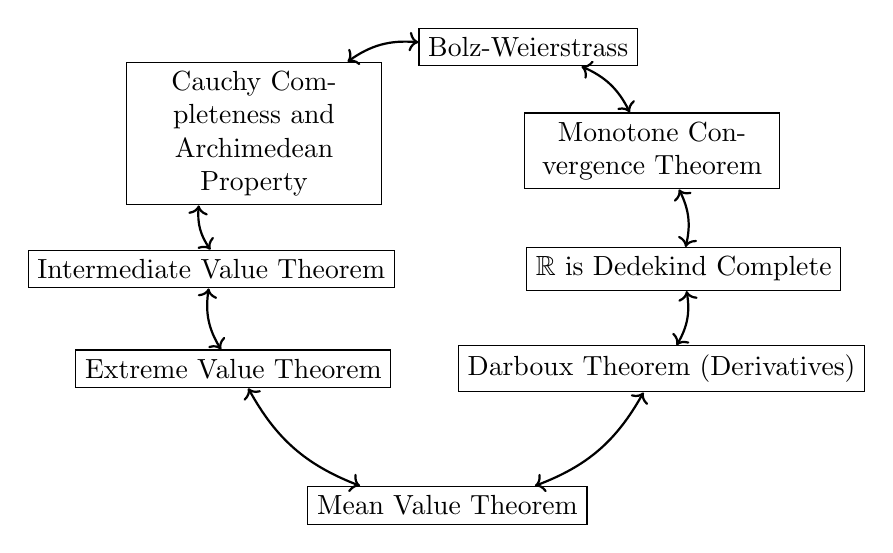
\begin{tikzpicture}
    % Set the radius for the circle of nodes
    \def\radius{3cm}
    % Define the 8 nodes with names in circular order
    \node[draw] (A) at (0:\radius) {$\mathbb{R}$ is Dedekind Complete};
    \node[draw, text width=3cm, align=center] (B) at (30:\radius) {Monotone Convergence Theorem};
    \node[draw] (C) at (70:\radius) {Bolz-Weierstrass};
    \node[draw, text width=3cm, align=center] (D) at (145:\radius) {Cauchy Completeness and Archimedean Property};
    \node[draw] (E) at (180:\radius) {Intermediate Value Theorem};
    \node[draw] (F) at (205:\radius) {Extreme Value Theorem};
    \node[draw] (G) at (270:\radius) {Mean Value Theorem};
    \node[draw] (H) at (335:\radius) {Darboux Theorem (Derivatives)};

    % Draw curved arrows (convex/outward) between adjacent nodes
    \foreach \from/\to in {A/B, B/C, C/D, D/E, E/F, F/G, G/H, H/A} {
        \draw[<->, bend right=20, thick] (\from) to (\to);
    }
\end{tikzpicture}

\newpage

\addcontentsline{toc}{section}{Chapter 1: The Real Number System}
\section*{Chapter 1: The Real Number System}

First remember, though we are following Rudin's book in these lectures, we are not covering the Complex Number System.

%%%%%%%%%%%%%%%%%%%%%%%%%%%%%%%%%%
%%% ADD NOTES ON RUDIN'S INTRO %%%
%%%%%%%%%%%%%%%%%%%%%%%%%%%%%%%%%%


\subsection{Ordered Sets}
Now we consider several important definitions. Most of these definitions will NOT be reiterated later on in this compilation. That being said, most of the content we cover will rely heavily on a total understanding of these definitions.\\

\textbf{Definition:} Let $S$ be a set. An \textcolor{ForestGreen}{order} on $S$ is a relation $<$ such that:
\begin{enumerate}
    \item \textcolor{ForestGreen}{Transitivity}: $a < b$ and $b < c \Longrightarrow a < c$
    \item \textcolor{ForestGreen}{Trichotomy}: Let $a,b,c \in S$. Then \textit{exactly} one of the following is true:
    \begin{enumerate}
        \item $a < b$
        \item $a = b$
        \item $b < a$
    \end{enumerate}
\end{enumerate}

Note that the above definition relied on another definition, given below:\\

\textbf{Definition}: Let $S$ be a set. A \textcolor{ForestGreen}{relation} is any subset of the cartesian product $S \times S$.\\

Further, some notes on notation:
\begin{enumerate}
    \item $y>x$ means $x<y$
    \item $x \leq y$ means $x < y$ \textit{or} $x = y$
    \item $x \geq y$ means $x > y$ \textit{or} $x = y$
\end{enumerate}

One example of an ordered set is the set of rational numbers, $\mathbb{Q} = \bigl\{a,b \in \mathbb{Z}, b \neq 0:\dfrac{a}{b}\bigr\}$.\\

\textbf{Definition}: Let $S$ be an ordered set and $E \subseteq S$. Say $E$ is \textcolor{ForestGreen}{bounded above} if $\exists \beta \in S:x \leq \beta \ \forall x \in E$. If so, $\beta$ is called an \textcolor{ForestGreen}{upper bound}.\\

Note that $\beta$ need not be an in $E$. Similarly, consider the definition for \textcolor{ForestGreen}{bounded below}:\\

\textbf{Definition}: Let $S$ be an ordered set and $E \subseteq S$. Say $E$ is \textcolor{ForestGreen}{bounded below} if $\exists \alpha \in S: \alpha \leq x \ \forall x \in E$. If so, $\alpha$ is called an \textcolor{ForestGreen}{lower bound}.\\

Again, note that $\alpha$ need not be in $E$.\\

\textbf{Definition}: Let $S$ be an ordered set. Let $E \subseteq S$ with $E$ bounded above. If $\exists \beta \in S$ such that:
\begin{enumerate}
    \item $\beta$ is an upper bound for $E$
    \item $\phi < \beta \Longrightarrow \phi$ is not an upper bound
\end{enumerate}

then $\beta$ is a \textcolor{ForestGreen}{least upper bound}, or \textcolor{ForestGreen}{supremum}.\\

\textbf{Definition}: Let $S$ be an ordered set. Let $E \subseteq S$ with $E$ bounded below. If $\exists \alpha \in S$ such that:
\begin{enumerate}
    \item $\alpha$ is a lower bound for $E$
    \item $\alpha < \rho \Longrightarrow \rho$ is not a lower bound
\end{enumerate}

then $\alpha$ is a \textcolor{ForestGreen}{greatest lower bound}, or \textcolor{ForestGreen}{infimum}.\\

\textbf{Definition}: An ordered set $S$ has the \textcolor{ForestGreen}{Least Upper Bound Property} if any nonempty subset which is bounded above has a least upper bound in $S$.\\

That is, $E \subseteq S$, $E \neq \emptyset$, and $E$ is bounded above $\Longrightarrow \sup{E} \in S$. Note that this Least Upper Bound Property (LUBP) is also referred to as \textcolor{ForestGreen}{Dedekind Completeness}.\\

For example, $\mathbb{Q}$ does not have LUBP ($\mathbb{Q}$ is not Dedekind Complete). To show this, let $E=\{q \in \mathbb{Q}: q^2 < 2\}$. Then $E \subseteq \mathbb{Q}$, $E \neq \emptyset$, and $E$ is bounded above, but $\sup{E}$ DNE. Consider \textcolor{blue}{Example 1.1} from Rudin:\\

Consider the equation $p^2=2$. We aim to show that $p \notin \mathbb{Q}$. To show this, assume $p \in \mathbb{Q}$. Then $p=\sfrac{m}{n}$ where $m,n \in \mathbb{Z}$ with $m$ and $n$ not both even. Then we have 

\begin{align*}
    p^2=2 &\Longrightarrow (\sfrac{m}{n})^2=2\\
    &\Longrightarrow \sfrac{m^2}{n^2}=2\\
    &\Longrightarrow m^2 = 2n^2 \\
    &\Longrightarrow m^2 \ \text{is even}\\
    &\Longrightarrow m \ \text{is even}\\
    &\Longrightarrow 4 \Divides m^2 \\
    &\Longrightarrow 4 \Divides 2n^2\\
    &\Longrightarrow n^2 \ \text{is even}\\
    &\Longrightarrow n \ \text{is even}.
\end{align*}

This is a contradiction, as we assumed that $m$ and $n$ are not both even. Then we must have that $p^2=2$ cannot be true for any $p \in \mathbb{Q}. \ \square$ \\

To examine further, let $A=\{p \in \mathbb{Q}^+:p^2 < 2\}$ and $B=\{p \in \mathbb{Q}^+:p^2 > 2\}$. Our aim is to show that \textit{$A$ contains no largest number and $B$ contains no smallest number}. More explicitly, for every $p \in A$ we can find a $q \in A$ such that $p < q$, and for every $p \in B$ we can find a $q \in B$ such that $q < p$. Then let us associate $q$ with each $p \in \mathbb{Q}^+$ such that 

\begin{center}
    $q = p - \dfrac{p^2-2}{p+2} = \dfrac{2p+2}{p+2}$.
\end{center}

Then we have 

\begin{center}
    $q^2-2=\dfrac{2(p^2-2)}{(p+2)^2} \ (*)$ .
\end{center}

By definition of set $A$, we have

\begin{align*}
    p \in A &\Longrightarrow p^2-2<0\\
    &\Longrightarrow q > p\\
    &\Longrightarrow q^2 < 2 \ \text{by} \ (*)\\
    &\Longrightarrow q \in A.
\end{align*}

Alternatively, 

\begin{align*}
    p \in B &\Longrightarrow p^2-2>0\\
    &\Longrightarrow 0<q<p\\
    &\Longrightarrow q^2>2 \ \text{by} \ (*)\\
    &\Longrightarrow q \in B. \ \square
\end{align*}

\textbf{Remark}: One way to interpret the example above is that the rational number system has certain gaps, even though there is always a rational number strictly between any two rational numbers: that is,

\begin{center}
    $r<s \Longrightarrow r< \dfrac{r+s}{2}<s$.
\end{center}

We have the real number system to fill these gaps.\\

\textbf{Theorem}: Every ordered set with LUBP also has the Greatest Lower Bound Property (GLBP).\\

\textit{Proof:} Let $S$ be an ordered set with LUBP. Let $B \subseteq S$, $B \neq \emptyset$, and $B$ is bounded below. Let $L = \{y \in S: y \leq x \ \forall x \in B\}$. That is, let $L$ be the set of all lower bounds for $B$.\\

\begin{tikzpicture}
    % Blue part of number line (left side), with arrow on the far left
    \draw[blue, latex-] (-3.5,0) -- (2, 0);
    
    % Orange part of number line (right side), with arrow on the far right
    \draw[orange, -latex] (2,0) -- (7.5, 0);

    % Tick marks
    \foreach \x in {-3,-2,-1,0,1,...,7}
        \draw (\x, 0.1) -- (\x, -0.1);

    % Colored tick and label for y (left side)
    \draw[blue] (-1, 0.1) -- (-1, -0.1) node[below, text=blue] {$y$};
    % Colored tick and label for x (right side)
    \draw[orange] (5, 0.1) -- (5, -0.1) node[below, text=orange] {$x$};

    % Labels above, also color-coded
    \node[above=0.25cm, text=blue] at (0,0) {$L$};
    \node[above=0.25cm, text=orange] at (4,0) {$B$};
    \node[below=.1cm] at (2,0) {\textbf{\textcolor{ForestGreen}{$\alpha$}}};
\end{tikzpicture}

Our goal is to find $\inf{B}$ as $\sup{L}$ since $L \subseteq S$ and all subsets of $S$ have LUBP.\\

First, note $L \neq \emptyset$ since $B$ is bounded below. By definition of $L$, $x$ is an upper bound for $L \ \forall x \in B$. Then $L$ is bounded above and by LUBP of $S$, $L$ has a supremum in $S$. Let $\alpha = \sup{L}$. Then we need to find $\alpha$. Then consider the following:

\begin{align*}
    x \in B &\Longrightarrow x \ \text{is an  upper bound for} \ L\\
    &\Longrightarrow \alpha \leq x \ \text{by definition of Supremum}\\
    &\Longrightarrow \alpha \ \text{is a lower bound for} \ B.
\end{align*}

Now, for sake of contradiction, suppose that $\beta$ is a lower bound for $B$ with $\beta > \alpha$. Then $\beta \in L$ and $\beta > \sup{L}$. But this is impossible, since $\sup{L}$ is an upper bound for $L$. Then $\alpha$ is the greatest lower bound for $B$ and thus, $S$ has GLBP. $\square$

\subsection{Fields}

\textbf{Definition}: A \textcolor{ForestGreen}{field} is a set $F$ with two binary oprations (addition and multiplication) that satisfies the following axioms for addition:

\begin{enumerate}
    \item $x,y \in F \Longrightarrow x+y \in F$ \ \textit{(closed under addition)}
    \item $x+y=y+x \ \forall x,y \in F$ \ \textit{(addition commutes)}
    \item $(x + y) + z = x + (y + z) \ \forall x,y,z \in F$ \ \textit{(addition is associative)}
    \item $0 \in F:0+x=x \ \forall x \in F$ \ \textit{($F$ contains an additive identity)}
    \item $x \in F \Longrightarrow -x \in F:x+(-x)=0$ \ \textit{($F$ contains additive inverses)}
\end{enumerate}

and the following axioms for multiplication:

\begin{enumerate}
    \item $x,y \in F \Longrightarrow xy \in F$ \ \textit{(closed under multiplication)}
    \item $xy=yx \ \forall x,y \in F$ \ \textit{(multiplication commutes)}
    \item $(xy)z=x(yz) \ \forall x,y,z \in F$ \ \textit{(multiplication is associative)}
    \item $1 \in F, 1 \neq 0:1x=x \ \forall x \in F$ \ \textit{($F$ contains a multiplicative identity)}
    \item $x \in F , x \neq 0\Longrightarrow \sfrac{1}{x} \in F: x \cdot (\sfrac{1}{x})=1 \in F$ \ \textit{($F$ contains multiplicative inverses)}.
\end{enumerate}

\textbf{Remarks}: The field axioms hold in $\mathbb{Q}$, so in turn $\mathbb{Q}$ is a field.\\

\textbf{Proposition 1.2.1}: \textit{The axioms for addition imply the following statements:}
\begin{enumerate}
    \item $x+y=x+z \Longrightarrow y = z$ \ \textit{cancellation law}
    \item $x+y=x \Longrightarrow y = 0$ \ \textit{additive identity is unique}
    \item $x+y=0 \Longrightarrow y = -x$ \ \textit{additive inverse is unique (on element by element basis)}
    \item $-(-x)=x$
\end{enumerate}

For each of the following proofs, let $F$ be a field with $x,y,z \in F$

\textbf{Proof} \textit{cancellation law}: Let $x+y=x+z$. Then we have
\begin{align*}
    y&=0+y\\
    &=(-x+x)+y\\
    &=-x+(x+y)\\
    &=-x+(x+z)\\
    &=(-x+x)+z\\
    &=0+z = z. \ \square 
\end{align*}

\textbf{Proof} \textit{additive identity is unique}: Let $x+y=x$. Then we have
\begin{align*}
    x+y=x &\Longrightarrow -x + (x + y) = -x + x\\
    &\Longrightarrow (-x+x)+y=-x+x\\
    &\Longrightarrow 0+y=0\\
    &\Longrightarrow y=0. \ \square 
\end{align*}

\textbf{Proof} \textit{additive inverse is unique (on element by element basis)}: Let $x+y=0$. Then we have
\begin{align*}
    x+y=0 &\Longrightarrow -x+(x+y)=-x+0\\
    &\Longrightarrow (-x+x)+y=-x\\
    &\Longrightarrow 0+y=-x\\
    &\Longrightarrow y=-x. \ \square
\end{align*}

\textbf{Proof} \textit{$-(-x)=x$}: \\

\textbf{Proposition 1.2.2}: \textit{The axioms for multiplication imply the following statements:}

\begin{enumerate}
    \item $x \neq 0, xy=xz \Longrightarrow y = z$ \textit{cancellation law}
    \item $x \neq 0, xy=x \Longrightarrow y = 1$ \ \textit{multiplicative identity is unique}
    \item $x \neq 0, xy=1 \Longrightarrow y=\sfrac{1}{x}$ \ \textit{multiplicative inverse is unique}
    \item $x \neq 0 \Longrightarrow \sfrac{1}{\sfrac{1}{x}}=x$.
\end{enumerate}

For each of the following proofs, let $F$ be a field with $x, y, z \in F$.\\

\textbf{Proof} \textit{cancellation law}: Let $xy=xz$ with $x \neq 0$. Then we have
\begin{align*}
    xy=xz &\Longrightarrow (\sfrac{1}{x})(xy)=(\sfrac{1}{x})(xz)\\
    &\Longrightarrow ((\sfrac{1}{x})x)y=((\sfrac{1}{x})x)z\\
    &\Longrightarrow 1y=1z\\
    &\Longrightarrow y=z. \ \square
\end{align*}

\textbf{Proof} \textit{multiplicative identity is unique}: Let $xy=x$ with $x \neq 0$. Then we have
\begin{align*}
    xy=x &\Longrightarrow (\sfrac{1}{x})(xy)=(\sfrac{1}{x})x\\
    &\Longrightarrow ((\sfrac{1}{x})x)y=1\\
    &\Longrightarrow 1y=1\\
    &\Longrightarrow y=1. \ \square
\end{align*}

\textbf{Proof} \textit{multiplicative inverse is unique}: Let $xy=1$ with $x \neq 0$. Then we have
\begin{align*}
    xy=1 &\Longrightarrow (\sfrac{1}{x})(xy)=(\sfrac{1}{x})1\\
    &=((\sfrac{1}{x})x)y=\sfrac{1}{x}\\
    &=1y=\sfrac{1}{x}\\
    &=y=\sfrac{1}{x}. \ \square
\end{align*}

\textbf{Proof} \textit{$x \neq 0 \Longrightarrow \sfrac{1}{\sfrac{1}{x}}=x$}:  \\

\textbf{Proposition 1.2.3} \textit{The field axioms imply the following statements, for any $x,y,z \in F$:}
\begin{enumerate}
    \item $0x=0$
    \item $x \neq 0, y \neq 0 \Longrightarrow xy \neq 0$
    \item $(-x)y = -(xy) =x(-y)$
    \item $(-x)(-y)=xy$
\end{enumerate}

\textbf{Proof} \textit{1.2.3-1}: $0x+0x=(0+0)x=0x$ \ by \textbf{1.2.1-2}. \ $\square$

\textbf{Proof} \textit{1.2.3-2}: We will prove this by contradiction. Let $x \neq 0, y \neq 0$, and assume $xy = 0$. Then we have 
\begin{center}
    $1=\biggl(\dfrac{1}{y}\biggr)\biggl(\dfrac{1}{x}\biggr)xy=\biggl(\dfrac{1}{y}\biggr)\biggl(\dfrac{1}{x}\biggr)0=0$.
\end{center}
But this is a contradiction, so we must have that $xy \neq 0$. \ $\square$

\textbf{Proof} \textit{1.2.3-3}: For the first equality, consider the following:
\begin{center}
    $(-x)y+xy=(-x+x)y=0y=0 \Longrightarrow (-x)y=-(xy)$.
\end{center}

The second equality is similar. Consider the following:
\begin{center}
    $x(-y)+xy=x(-y+y)=x \cdot 0 = 0 \Longrightarrow x(-y)=-(xy)$. \ $\square$
\end{center}

\textbf{Proof} \textit{1.2.3-4}: Consider the following:
\begin{center}
    $(-x)(-y)=-[x(-y)]=-[-(xy)]=xy$. \ $\square$
\end{center}

\textbf{Definition:} An \textcolor{ForestGreen}{ordered field} is a field $F$ which is an ordered set and holds the following properties:
\begin{enumerate}
    \item $x,y,z \in F, y < z \Longrightarrow y+x<z+x$ \ (note that this also holds for left addition), and 
    \item $x,y \in F, x>0, y>0 \Longrightarrow xy>0$. 
\end{enumerate}

A couple of notes on the above definition:
\begin{enumerate}
    \item Each of the properties listed give us that ordering is compatible with addition and multiplication, respectively.
    \item Statements like $a>0, a \in F$ are used with the understanding that $0$ is the additive identity in $F$.
    \item $x>0 \Longrightarrow x$ \ is "positive" and $x<0 \Longrightarrow x$ \ is "negative". This concept works for other structures like matrices, for example.
\end{enumerate}

One example of an ordered field is $\mathbb{Q}$. Some examples of sets that are NOT ordered fields are $\mathbb{Z}$ (since $\mathbb{Z}$ is not a field) and $\mathbb{C}$ (since $\mathbb{C}$ is not ordered.\\

\textbf{Proposition 1.2.4} \textit{The following statements are true in every ordered field}:
\begin{enumerate}
    \item $x>0 \Longrightarrow -x<0$ \ and vice versa,
    \item $x > 0, y < z \Longrightarrow xy<xz$,
    \item $x<0,y<z \Longrightarrow xy>xz$
    \item $x \neq 0 \Longrightarrow x^2>0$. In particular, $1>0$.
    \item $0<x<y \Longrightarrow 0<\sfrac{1}{y} < \sfrac{1}{x}$
\end{enumerate}

\textbf{Proof} \textit{1.2.4-1}: Let $x>0$. Then we have
\begin{align*}
    x>0 &\Longrightarrow 0=-x+x>-x+0\\
    &\Longrightarrow -x<0.
\end{align*}
Now, if $x<0$, then we have 
\begin{align*}
    x<0&\Longrightarrow 0=-x+x<-x+0\\
    &\Longrightarrow -x>0. \ \square
\end{align*}

\textbf{Proof} \textit{1.2.4-2} Let $x>0$ and $y<z$. Then we have
\begin{align*}
    y<z &\Longrightarrow 0=y-y<z-y\\
    &\Longrightarrow 0<x(z-y)\\
    &\Longrightarrow xy=0+xy<x(z-y)+xy=xz. \ \square
\end{align*}

\textbf{Proof} \textit{1.2.4-3} Let $x<0$ and $y<z$. Then we have
\begin{center}
    $-[x(z-y)]=(-x)(z-y)>0 \Longrightarrow x(z-y)<0 \Longrightarrow xz<xy$. \ $\square$
\end{center}

\textbf{Proof} \textit{1.2.4-4} Let $x\neq 0$. Then we consider two cases: $x>0$ and $x<0$. First, the former:
\begin{center}
    $x>0 \Longrightarrow x^2>0$
\end{center}
by definition of an ordered field. For the latter, we have:
\begin{center}
    $x<0 \Longrightarrow -x>0 \Longrightarrow (-x)^2>0$.
\end{center}
But $x^2=(-x)^2$ by \textbf{Proposition 1.2.3-4}. Since $1=1^2$, we must have $1>0$. \ $\square$

\textbf{Proof} \textit{1.2.4-5} Let $0<x<y$. Specifically, let $y>0$ and also let $v \leq 0$. Then we must have $yv \leq 0$. But $y \cdot (\sfrac{1}{y})=1>0 \Longrightarrow \sfrac{1}{y}>0$. Likewise, $\sfrac{1}{x}>0$.Then consider the following:
\begin{align*}
    x<y &\Longrightarrow (\sfrac{1}{x})(\sfrac{1}{y})x<(\sfrac{1}{x})(\sfrac{1}{y})y\\
    &\Longrightarrow (\sfrac{1}{y})(\sfrac{1}{x})x<(\sfrac{1}{x})((\sfrac{1}{y})y)\\
    &\Longrightarrow (\sfrac{1}{y})((\sfrac{1}{x})x)<(\sfrac{1}{x})((\sfrac{1}{y})y)\\
    &\Longrightarrow (\sfrac{1}{y})\cdot 1<(\sfrac{1}{x})\cdot 1\\
    &\Longrightarrow \sfrac{1}{y}<\sfrac{1}{x}. \ \square
\end{align*}

\subsection{The Real Field}

Constructing fields might seem intimidating, but this process is necessary for understanding $\mathbb{R}$. $\mathbb{Q}$ is easy to construct from $\mathbb{N}$. Further, there are many ways to construct $\mathbb{R}$ from $\mathbb{Q}$. The most common ways are Dedekind cuts or equivalence classes of Cauchy Sequences of rationals. Note that this process will be seen at the end of the semester. %see chapter 1 dedekind cuts appendix p17%\\

Along the way one proves:\\

\textbf{Theorem 1.3.1}: There exists a unique (up to isomorphism) ordered field (namely, $\mathbb{R}$), containing an ordered subfield, $\mathbb{Q}$, with LUBP.\\

This can be similarly stated as there exists a unique (up to isomorphism) complete (Dedekind complete) ordered field.

\textbf{Theorem 1.3.2}: The following two items are known as the \textcolor{ForestGreen}{Archimedian Property} and the \textcolor{ForestGreen}{density} of $\mathbb{Q}$:
\begin{enumerate}
    \item $\forall x,y \in \mathbb{R}, x>0, \exists n \in \mathbb{N}: nx>y$
    \item $\forall x,y \in \mathbb{R}, x<y, \exists p \in \mathbb{Q}:x<p<y$.
\end{enumerate}

\textbf{Proof} \textit{1.3.2-1} First, we will show $\forall z >0, \exists n \in \mathbb{N}: n>z$. For sake of contradiction, assume $\mathbb{N}$ is bounded above. Then, by LUBP of $\mathbb{R}, \exists \alpha \in \mathbb{R}: \alpha=sup\mathbb{N}$. \\

Now, since $\alpha - 1 < LUB$, we have that $\alpha - 1 < \alpha \Longrightarrow \alpha - 1$ is not an upper bound for $\mathbb{N}$. Then we must have that there exists a natural number $m$ such that $m>\alpha - 1$. But, alas, this implies that $\alpha < m+1$ and $m + 1 \in \mathbb{N}$. This contradicts $\alpha$ being an upper bound for $\mathbb{N}$. Now, let $z = \frac{y}{x} \Longrightarrow z < n$. \ $\square$\\

Before we start the proof of \textbf{1.3.2-2}, we will note a useful definition:\\

\textbf{Definition:} The \textcolor{ForestGreen}{Well-Ordering Principle} states that every nonempty subset of $\mathbb{N}$ has a least number or element.

\textbf{Proof} \textit{1.3.2-2} For the first case, assume $x \geq 0$. Now, $y-x>0$. By \textbf{1.3.2-1}, $\exists n \in \mathbb{N}:n(y-x)>1$. Also by \textbf{1.3.2-1}, $\exists k \in \mathbb{N}: k>nx$. This shows the set $A=\{k \in \mathbb{N}: k>nx\}$ is nonempty. \\

By the Well-Ordering Principle, $A$ has a least number $m$. Then we have

\begin{align*}
    m-1 \notin A &\Longrightarrow m-1 \leq nx <m \\
    &\Longrightarrow m \leq nx+1 <m+1\\
    &\Longrightarrow nx<m\leq nx+1<nx+n(y-x)=ny\\
    &\Longrightarrow x<\dfrac{m}{n} <y.
\end{align*}

Note that in the statement above, $\dfrac{m}{n}$ is the $p$ from the theorem which we are proving.

Next, we assume $x<0$. Then this leads to two sub-cases:
\begin{enumerate}
    \item $y>0 \Longrightarrow p=0$ works, since $0 \in \mathbb{Q}$ and $x<0<y$.
    \item Assume $y \leq 0$. Then $0 \leq -y < -x$. By the first assumption, $\exists p \in \mathbb{Q}:-y<p<-x \Longrightarrow x < -p < y. \ \square$ 
\end{enumerate}

Note that in the second sub-case above, if $p \in \mathbb{Q}$, we must have that $-p \in \mathbb{Q}$.\\

\textbf{Corollary 1.3.3} Let $x,y \in \mathbb{R}, x < y$. Then $\exists \rho \in \mathbb{Q}^c:x<\rho<y$.\\

\textbf{Proof} Let $x,y \in \mathbb{R} \ \text{with} \ x < y$. Then 
\begin{align*}
    x < y &\Longrightarrow \dfrac{x}{\sqrt{2}} < \dfrac{y}{\sqrt{2}}\\
    &\Longrightarrow \dfrac{x}{\sqrt{2}} < q < \dfrac{y}{\sqrt{2}} \ \text{with} \ q \in \mathbb{Q}\\
    &\Longrightarrow x < q\sqrt{2} < y. \ \square
\end{align*}

Note that $q\sqrt{2}$ is irrational (this can be shown with the same method used in \textcolor{blue}{Example 1.1} from Rudin.\\

\textbf{Theorem 1.3.4} Let $x \in \mathbb{R}^+$ and $n \in \mathbb{N}$. Then $\exists ! y \in \mathbb{R}^+:y^n=x$.\\

Note that we can write $y=\sqrt[n]{x}$ or $y=x^{\sfrac{1}{n}}$ to express the same result as $y^n=x$. Further, it should be known that $\exists!y$ means that there exists a \textit{unique} $y$. Also note that the above theorem states that $\mathbb{R}^+$ is closed under roots.\\

\textbf{Proof} First, we will prove uniqueness (by contradiction). Assume $y_1^n=x$ and $y_2^n=x$. Then, by trichotomy, either $y_1=y_2, y_1>y_2,$ or $y_1<y_2$. Without loss of generality, assume $y_1<y_2$. Then we must have that $y_1^n<y_2^n$, and thus we have a contradiction, whence $y_1=y_2$.\\

Next, we will prove existence of such a $y$. Let $E=\{t \in \mathbb{R}^+:t^n<x\}$.\\

\begin{tikzpicture}
     % Blue part of number line (left side), with arrow on the far left
    \draw[ForestGreen, latex-] (-3.5,0) -- (2, 0);
    
    % Black part of number line (right side), with arrow on the far right
    \draw[-latex] (2,0) -- (7.5, 0);

    % Tick marks
    \foreach \x in {-3,-2,-1,0,1,...,7}
        \draw (\x, 0.1) -- (\x, -0.1);

    % Colored tick and label for y (left side)
    

    % Label below, also color-coded
    \node[below=.1cm] at (2,0) {\textbf{\textcolor{ForestGreen}{$\sqrt{x}$}}};
\end{tikzpicture}

Let $t = \dfrac{x}{1+x}$. Then we have 

\begin{align*}
    t=\dfrac{x}{1+x} &\Longrightarrow 0<t<1\\
    &\Longrightarrow t^n<t<x \\
    &\Longrightarrow t \in E\\
    &\Longrightarrow E \neq \emptyset.
\end{align*}

Now, we choose a different $t > 1+x$ with $x$ fixed. Then, since $t> 1+x$, we have

\begin{align*}
    t > 1+x &\Longrightarrow t>1\\
    &\Longrightarrow t^n>t \ \text{and} \ t>x\\
    &\Longrightarrow t \notin E
\end{align*}

Then the contrapositive states that $t \in E \Longrightarrow t \leq 1+x$ and thus $1+x$ is an upper bound for $E$. That is, $E$ is bounded above.\\

By the Least Upper Bound Property of $\mathbb{R}$, $\exists y \in \mathbb{R}:y=\sup{E}$. Here, we will choose our $y$ such that $y^n=x$. First, algebra: 
\begin{center}
    $b^n-a^n=(b-a)(b^{n-1}+b^{n-2}a+b^{n-3}a^2+ \cdots + ba^{n-2}+a^{n-1})$.
\end{center}

In particular, if $0<a<b$, then we must have that 

\begin{center}
    $b^n-a^n<(b-a)nb^{n-1}$ $(*)$
\end{center}

For sake of contraduction, assume $y^n<x$. Then choose $h \in (0,1)$ such that $h < \dfrac{x-y^n}{n(y+1)^{n-1}}$. In particular, we choose $h$ to be the minimum of these two conditions.\\

If we let $a=y$ and $b=y+h$ in $(*)$, we have 

\begin{align*}
    (y+h)^n-y^n &< hn(y+h)^{n-1}\\
    &<hn(y+1)^{n-1} \ \text{(since} \ h<1)\\
    &< hn(y+1)^{n-1}\\
    &<x-y^n \ \biggl(\text{since} \ h < \dfrac{x-y^n}{n(y+1)^{n-1}}\biggr).
\end{align*}

Thus $(y+h)^n < x$ and so $(y+h) \in E$. But $y>0 \Longrightarrow y+h>y=\sup{E}$. This is a contradiction, as $\sup{E}$ is an upper bound. Then we must have that $y^n \not<x$. \\

Now, for sake of contradiction, assume $y^n>x$. Let $k=\dfrac{y^n-x}{ny^{n-1}}$, so $k>0$. Since $k=\dfrac{y}{n}-\dfrac{x}{ny^{n-1}}$ and $\dfrac{y}{n} \leq y$, we see that $k<y$. Now choose $t \geq y-k > 0$. Then 

\begin{align*}
    y^n-t^n &\leq y^n-(y-k)^n \ \text{(since} \ t\geq y-k)\\ 
    &< kny^{n-1} \ \text{by} \ (*) \ \text{with} \ b=y, a=y-k\\ 
    &=y^n-x \ \text{by definition of k}.
\end{align*}

Then $t^n>x \Longrightarrow t \notin E$. Then we just showed that $t \geq y-k \Longrightarrow t \notin E$. But $t \in E \Longrightarrow t < y-k$, ergo $y-k$ is an upper bound for $E$. But $y-k<y$, which contradicts $y=\sup{E}$ as the \textit{least} upper bound. So then $y^n \not> x$, and thus $y=x^n$. \ $\square$

\newpage

\addcontentsline{toc}{section}{Chapter 2: Basic Topology}
\section*{Chapter 2: Basic Topology}
\setcounter{section}{2}
\setcounter{subsection}{0}
\subsection{Finite, Countable, and Uncountable Sets}

\textbf{Definition:} If $A$ and $B$ are sets and there exists a bijection $f:A \longrightarrow B$, then $A$ and $B$ have the same \textcolor{ForestGreen}{cardinality}, and we write $|A|=|B|$. Note that we can easily check that this is an equivalence relation:

\textbf{Proof:} Let $A,B$ and $C$ be sets such that $|A|=|B|=|C|$. First, note that the identity map $id_A:A \longrightarrow A$ is bijective, as it is a map onto itself. Next, let $f:A \longrightarrow B$ be a bijection of $A$ onto $B$ (since $|A|=|B|$. Then the inverse map of $f$, $f^{-1}:B \longrightarrow A$ is a bijection of $B$ onto $A$. Lastly, consider two bijections $f$ and $g$ with $f: A \longrightarrow B$ and $g: B \longrightarrow C$. Then the composition of these functions $g \circ f$ is a bijection of $A$ onto $C$. Then we must have that cardinality is an equivalence relation. $\square$\\

\textbf{Definition:} If $|A|=|\{1,2,3, \dots,n\}|$ for some $n \in \mathbb{N}$, then $A$ is \textcolor{ForestGreen}{finite}, and we write $|A|=n$. If $A$ is not finite, then $A$ is \textcolor{ForestGreen}{infinite}.\\

\textbf{Definition:} If $|A|=|\mathbb{N}|$, then we say $A$ is \textcolor{ForestGreen}{countably infinite}. If $A$ is countably infinite or finite, then $A$ is \textcolor{ForestGreen}{at most countable}. The term "countable" can refer to either of these. We only use this informally or when it doesn't matter. If $A$ is finite but not countable, then $A$ is \textcolor{ForestGreen}{uncountable}.\\

Note that \textcolor{ForestGreen}{Cantor-Schroder-Bernstein Theorem} states:\\

If there exist injections $f:A \longrightarrow B$ and $g: B \longrightarrow A$, then $|A|=|B|$. We will not prove or use this during the current course, but it can be a fun exercise.\\

Also note that one common notation for the existence of an injection $f:A \longrightarrow B$ is $|A| \leq |B|$.

\textbf{Definition:} Dedekind defined infinite by saying that $A$ is infinite if $\exists B \subsetneq A$ with $|B|=|A|$.\\

\textbf{\textcolor{Blue}{Example 2.1}:} $\mathbb{Z}$ is countable. Let $f: \mathbb{N} \longrightarrow \mathbb{Z}$ be given by 

\begin{center}
    \[
f(n) = 
\begin{cases}
\dfrac{n}{2}, & \text{if } n \ \text{even} \\
-\dfrac{n-1}{2}, & \text{if } n \ \text{odd.}
\end{cases}
\]
\end{center}

It is easy to check that this is a bijection, so we have that $|\mathbb{Z}|=|\mathbb{N}|$. Further, note that $\mathbb{N} \subsetneq \mathbb{Z}$, so $\mathbb{Z}$ is Dedekind infinite.

\textbf{Definition:} A \textcolor{ForestGreen}{sequence} is a function $f: \mathbb{N} \longrightarrow A$ where $A$ is a set. Usually, we write $X_n$ or $a_n$ for $f(n)$ and we write $\{x_n\}$ or $(a_n)$ for the function itself. Then $\{x_n\}$ is \textit{not} a set. Specifically, $\{x_n\} \nsubseteq A$. Some important distinctions between sets and functions are that order matters in a set (this is the ordering of elements, not order relating to cardinality) and sets can't repeat elements. \\

One last note: the \textcolor{ForestGreen}{range}, or \textcolor{ForestGreen}{image} $\{x_n \Divides n \in \mathbb{N}\}$ \textit{is} a set. Specifically, the range is a subset of $A$ and is \textit{always} at-most countable. That is, the range is \textit{never} uncountable. Further, every at-most countable set is the range of some sequence.

\textbf{Theorem 2.1:} Every infinite subset of a countable set is countable. (Note that this infinite subset is the \textit{smallest} infinity.

\textbf{Proof:} Suppose $A$ is countably infinite and $E \subseteq A$ is infinite. Then we arrange the elements of $A$ in a sequence $\{a_n\}$ by constructing \textit{(always using the \textcolor{ForestGreen}{axiom of choice})} in $E$ as follows:\\

let $n_1 \in \mathbb{N}$ be the smallest natural number: $a_{n_1} \in E$. For $k \geq 2$, let $n_k \in \mathbb{N}$ be the smallest natural number greater than $n_{k-1}:a_{n_k} \in E$. The sequence $f(k)=a_{n_k}$ \textit{(which is a subsequence by the \textcolor{ForestGreen}{Bolzano Weierstrass theorem})} is a bijection from $\mathbb{N}$ to $E. \ \square$

Note that we just showed that countable is the smallest infinity. Also note that if $A$ is countable, then we must have that any subset $E \subseteq A$ is also countable. This second note is important, as we will use the contrapositive of this statement often. 

\begin{center}
    $\exists E \subseteq A: E \ \text{uncountable} \Longrightarrow A \ \text{uncountable}$
\end{center}

\textbf{Definition:} Let $A, \Omega$ be sets. Assume $\exists f:A \longrightarrow \mathcal{P}(\Omega)$ where $\mathcal{P}(\Omega)$ is the \textcolor{ForestGreen}{power set} of $\Omega$ \textit{(a.k.a. $2^{\Omega}$)}. For $\alpha \in A$, denote $f(\alpha)$ by $E_{\alpha}$, and note that $E_{\alpha} \subseteq \Omega$. The image $f(A)$ is denoted $\{E_{\alpha}\}$ and is usually called a \textcolor{ForestGreen}{collection} or \textcolor{ForestGreen}{family} of subsets of $\Omega$. We also write

\begin{align*}
    \bigcup_{\alpha \in A} E_{\alpha} &= \{x:x \in E_{\alpha}, \exists \alpha \in A\}\\
    \bigcap_{\alpha \in A} E_{\alpha} &= \{x:x \in E_{\alpha}, \forall \alpha \in A\}.
\end{align*}

\textbf{Theorem 2.2: \textcolor{ForestGreen}{De Morgan's Laws}}
\begin{align*}
    \left(\bigcup_{\alpha \in A} E_{\alpha} \right)^c &= \bigcap_{\alpha \in A} E_{\alpha} ^c\\
    \left(\bigcap_{\alpha \in A} E_{\alpha} \right)^c &= \bigcup_{\alpha \in A} E_{\alpha} ^c
\end{align*}

The proof of this theorem is left as an exercise.

\begin{table}[H]
\centering
\begin{tabular}{|c|c|c|}
  \hline
  logic & set theory & algebra \\
  \hline
  $\lor$ & $\bigcup$ & $+$ \\
  \hline
  $\land$ & $\bigcap$ & $\cdot$ \\
  \hline
\end{tabular}
\caption{Philosophical Logic Notation}
\end{table}

Note that the columns for logic and set theory above are literally true, while the columns between set theory and algebra are superficially true.

\begin{table}[H]
\centering
\begin{tabular}{|p{5cm}|p{3.9cm}|p{4cm}|}
    \hline
    \textbf{Set Theory} & \textbf{Algebra} & \textbf{Rule/Law} \\
    \hline
    $A \cup B = B \cup A$ & $a + b = b + a$ & Commutativity \\
    \hline 
    $A \cap B = B \cap A$ & $ab = ba$ & Commutativity \\
    \hline 
    $A \cup (B \cup C) = (A \cup B) \cup C$ & $a + (b + c) = (a + b) + c$ & Associativity \\
    \hline
    $A \cap (B \cap C) = (A \cap B) \cap C$ & $a(bc) = (ab)c$ & Associativity \\
    \hline 
    $A \cap (B \cup C) = (A \cap B) \cup (A \cap C)$ & $a(b + c) = ab+ac$ & Distributivity \\
    \hline
    $A \cup \emptyset = A$ & $a+0=a$ & Additive Identity Under Addition/Union\\
    \hline
    $A \cap \emptyset = \emptyset$ & $a \cdot 0 = 0$ & Additive Identity Under Multiplication/Intersection\\
    \hline
\end{tabular}
\caption{Set Theory and Algebraic Analogies}
\end{table}

Still, we must be careful with ordering:

\begin{table}[H]
\centering
\begin{tabular}{|p{5cm}|p{3.9cm}|p{4cm}|}
    \hline
    \textbf{Set Theory} & \textbf{Algebra} & \textbf{Condition} \\
    \hline
    $A \subseteq A \cup B$ is true & $a \leq a+b$ is true & if $b \geq 0$ \\
    \hline 
    $A \cap B \subseteq A$ is true & $ab \leq a$ is false & unless $b < 1$\\
    \hline
    $A \subseteq B \Longrightarrow A \cup B=B$ & $a \leq b \Longrightarrow a+b=b$ is false & unless $a=0$\\
    \hline
    $A \subseteq B \Longrightarrow A \cap B = A$ & $a \leq b \Longrightarrow ab=a$ is false & unless $b=1$ or $a = 0$\\
    \hline 
\end{tabular}
\caption{Ordering Irregularities}
\end{table}

The proofs of the left side are left as exercises to the reader.

\textbf{Theorem 2.3:} A countable union of countable sets is countable.

\textbf{Proof:} Let $E_n$ be countable for all $n \in \mathbb{N}$. We will arrange each $E_n$ in a sequence $\{x_{n,k}\}$. Consider the array below:

\[
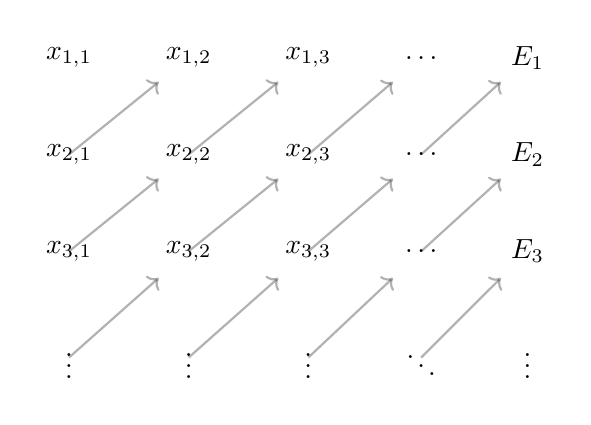
\begin{tikzpicture}[baseline=(m.center)]

\matrix (m) [matrix of math nodes, nodes={anchor=center}, row sep=2em, column sep=2em] {
  x_{1,1} & x_{1,2} & x_{1,3} & \dots & E_1 \\
  x_{2,1} & x_{2,2} & x_{2,3} & \dots & E_2 \\
  x_{3,1} & x_{3,2} & x_{3,3} & \dots & E_3 \\
  \vdots & \vdots & \vdots & \ddots & \vdots \\
};

% Arrow length scale (1 = full length, <1 = shorter arrows)
\def\scale{0.75}

\foreach \r in {2,3,4} {
  \foreach \c in {1,2,3,4} {
    \draw[->, thick, opacity=0.3] 
      let 
        \p1 = (m-\r-\c.center), 
        \p2 = (m-\the\numexpr\r-1\relax-\the\numexpr\c+1\relax.center),
        \n1 = {(\x2-\x1)*\scale},
        \n2 = {(\y2-\y1)*\scale}
      in
        (\x1,\y1) -- ++(\n1,\n2);
  }
}

\end{tikzpicture}
\]

Clearly, every element of $\bigcup_{n \in \mathbb{N}} E_n$ appears in the array. Then we create a new sequence $\{y_m\}=\{x_{1,1}, x_{2,1}, x_{1,2}, x_{3,1}, x_{2,2}, x_{1,3}, \dots \}$. This new sequence \textcolor{ForestGreen}{enumerates} $\bigcup_{n \in \mathbb{N}} E_n. \ \square$

Note: We assume $E_n$ is countably infinite here. If some $E_n$ or $A$ is finite, it is easy to modify the proof accordingly.

\textbf{Corollary:} A finite union of countable sets is countable, and a countable union of finite sets is countable.

\textbf{Theorem 2.4:} Let $A$ be a countable set. Then $A^n = A \times A \times \dots \times A = \prod_{k=1}^{n} A_n$ is countable. Note that this is the \textcolor{ForestGreen}{cartesian product} of each $A_k$.

\textbf{Proof:} We will prove by induction (\textit{this might be the only time we EVER use induction}). First, the case for $n=1$ is trivial (\textit{note that using the word trivial will also be exceedingly rare in this course}). \\
Now, assume $A^n$ is countable. We need to show that $A^{n+1}$ is countable. We have

\begin{align*}
    A^{n+1} &= \{(a_1,a_2, \dots,a_n,a_{n+1}) \Divides a_i \in A \ \forall i\}\\
    &=\{(b, a_n+1) \Divides b \in A^n, a_{n+1} \in A\}\\
    &= \bigcup_{b \in A^n} \{(b,a_{n+1}) \Divides a_n+1 \in A\} \ \textit{note that here $b$ is fixed}\\
    &= \bigcup_{a_{n+1} \in A} \{(b,a_{n+1}) \Divides b \in A^n\} \ \textit{this is equivalent to the line above}.
\end{align*}

But for a fixed $b \in A^n$, $\{(b,a_{n+1}) \Divides a_{n+1} \in A\}$ is clearly bijective with $A$ itself, and is therefore countable. Then $A^{n+1}$ is a countable union of countable sets. So $A^{n+1}$ is countable by \textbf{Theorem 2.3}. $\square$

\textbf{Corollary 2.1:} $\mathbb{Q}$ is countable.\\
\textbf{Proof:} \textit{(informal)} Think of $\mathbb{Q}$ as a subset of $\mathbb{Z} \times \mathbb{Z}$. Then by one of our theorems above, $\mathbb{Z} \times \mathbb{Z}$ is countable. Then by another theorem above, $\mathbb{Q}$ is countable. $\square$

\textbf{Theorem 2.5:} The \textcolor{ForestGreen}{set of binary sequences} is uncountable. Note that the set of binary sequences is a set where each element is a sequence. That is,

\begin{center}
    $\bigl\{ \{x_n\} \Divides x_n \in \{0,1\} \ \forall n \in \mathbb{N} \bigr\}$
\end{center}

Note that, in the definition above, $\{x_n\}$ is a sequence and $\{0,1\}$ is a set.

\textbf{Proof:} For sake of contradiction, suppose $\{a_k\}$ is a sequence of \textit{all} binary sequences. Suppose $a_k=\{a_{k,1},a_{k,2},a_{k,3}, \dots\}$, where $a_{k,i} \in \{0,1\} \ \forall k,i \in \mathbb{N}$. Let 
\[
b_n = \begin{cases}
    0, & \text{if } a_{n,n} = 1 \\
    1, & \text{if } a_{n,n} = 0.
\end{cases}
\]

Note that $b_n$ is all of the diagonal elements \textit{(see array below):}

\[
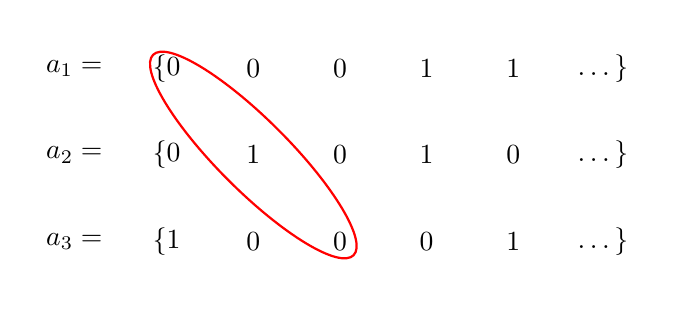
\begin{tikzpicture}[baseline=(m.center)]
  % Matrix setup
  \matrix (m) [matrix of math nodes,
               nodes={minimum width=8mm, minimum height=8mm, anchor=center},
               column sep=3mm, row sep=3mm]
  {
    a_{1} = & \{0 & 0 & 0 & 1 & 1 & \dots\} \\
    a_{2} = & \{0 & 1 & 0 & 1 & 0 & \dots\} \\
    a_{3} = & \{1 & 0 & 0 & 0 & 1 & \dots\} \\
  };

  % Coordinates of the three cells to cover
  \coordinate (start) at (m-1-2.center);
  \coordinate (end) at (m-3-4.center);

  % Calculate center point between start and end
  \path let \p1 = (start), \p2 = (end) in
    coordinate (center) at ($(\p1)!.5!(\p2)$);

  % Draw rotated ellipse centered between start and end, rotated -45 degrees
  \draw[red, thick]
    (center) ellipse [x radius=18mm, y radius=4.5mm, rotate=-45];
\end{tikzpicture}
\]

Note that, in the array example above, $b_n=\{1 \ 0 \ 1 \ \dots\}$. Then $\{b_n\}$ is a binary sequence. But this $\{b_n\}$ does \textit{not} appear in $\{a_k\}$ since $b_{i,i} \neq a_{i,i}$ for any $i \in \mathbb{N}$. This contradicts that $\{a_k\}$ contains \textit{all} binary sequences. $\square$

Note that this is a standard comprehensive exam problem. The argument we used is called \textcolor{ForestGreen}{Cantor's Diagonal Argument}. There are many variations of this argument. We used it to try to write the set as a sequence. Note that a set is only countable if and only if it can be written as a sequence (enumerated).

\textbf{Corollary 2.2:} The interval $[0,0.2)$ is uncountable.

\textbf{Proof:} Let $f$ be a function such that 

\begin{align*}
    f:&\{\text{binary sequences}\} \longrightarrow [0,0.2)\\
    &\{a_1, a_2, a_3, \dots \} \longmapsto 0.a_1 a_2 a_3 \dots .
\end{align*}

Then $f$ is clearly injective, so $Im(f)$ \textit{(image, range)} is uncountable. Since $Im(f) \subseteq [0,0.2)$, by the previous theorem, $[0,0.2)$ is uncountable. $\square$

Note that $f:\{\text{binary sequences}\} \longrightarrow [0,0.2)$ is injective but not surjective. Also, note that $f:\{\text{binary sequences}\} \longrightarrow Im(f)$ is bijective.

\textbf{Corollary:} $\mathbb{R}$ is uncountable.
\textbf{Proof:} $[0,0.2) \subseteq \mathbb{R}$. $\square$

Note that it is common to modify the diagonal argument to show that $(0,1)$ is uncountable. Then we can use a linear bijection to get $|(0,1)|=\left|\left(-\dfrac{\pi}{2},\dfrac{\pi}{2}\right)\right|$. After, we can use a bijection $\tan:\left(-\dfrac{\pi}{2},\dfrac{\pi}{2}\right) \longrightarrow \mathbb{R}$ to get $\left|\left(-\dfrac{\pi}{2},\dfrac{\pi}{2}\right)\right|=|\mathbb{R}|$.

Also, note that we showed $\prod_{i=1}^{\infty} \{0,1\}$ is uncountable \textit{(all binary strings/sequences)}. Then countable products of countable (finite) sets are \textit{not} countable. It is also important to note that products behave differently than unions.

\newpage

\subsection{Metric Spaces}

\textbf{Definition:} A \textcolor{ForestGreen}{metric space} is a pair $(X,d)$ where $X$ is a set and $d: X \times X \longrightarrow \mathbb{R}$ is a function (metric) satisfying:

\begin{enumerate}
    \item $d(x,y) \geq 0$ with $d(x,y)=0$ iff $x=y$ (positive definite)
    \item $d(x,y)=d(y,x)$ (symmertric)
    \item $d(x,y) \leq d(x,z) + d(z,y)$ (triangle inequality
\end{enumerate}

for all $x,y,z \in X$.

\textbf{Examples:}
\begin{enumerate}
    \item Let $X = \mathbb{R}$. Then
    \begin{enumerate}
        \item $d(x,y) = |x-y|$ is the \textcolor{ForestGreen}{"standard metric"}\\
        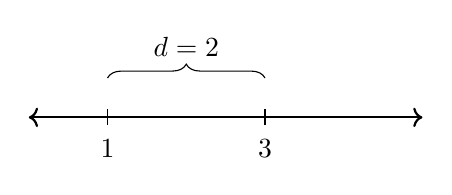
\begin{tikzpicture}
            \draw[thick, <->] (0,0) -- (5,0);
    
            % Tick marks and labels
            \foreach \x in {1, 3} {
            \draw (\x, 0.1) -- (\x, -0.1);
            \node at (\x, -0.4) {\x};
            }

            % Curly brace and label
            \draw [decorate, decoration={brace, amplitude=5pt}, yshift=0.5cm]
            (1,0) -- (3,0) node[midway, yshift=0.4cm] {$d = 2$};
        \end{tikzpicture}
        \item \[
d(x,y) = \dfrac{|x-y|}{|x-y|+1}
\]

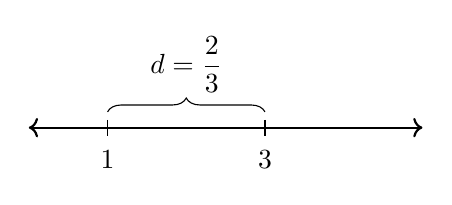
\begin{tikzpicture}
    \draw[thick, <->] (0,0) -- (5,0);

    % Tick marks and labels
    \foreach \x in {1, 3} {
        \draw (\x, 0.1) -- (\x, -0.1);
        \node at (\x, -0.4) {\x};
    }

    % Curly brace and label
    \draw [decorate, decoration={brace, amplitude=5pt}, yshift=0.2cm]
        (1,0) -- (3,0) node[midway, yshift=0.6cm] {$d = \dfrac{2}{3}$};
\end{tikzpicture}

        \item

\[
d(x,y) = \begin{cases}
    0, & \text{if } x=y \\
    1, & \text{if } x \neq y.
\end{cases}
\]

\begin{center}
    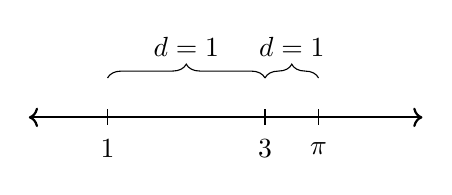
\begin{tikzpicture}
        \draw[thick, <->] (0,0) -- (5,0);

        % Tick marks and labels
        \foreach \x in {1, 3} {
            \draw (\x, 0.1) -- (\x, -0.1);
            \node at (\x, -0.4) {\x};
        }

        \draw (3.68, 0.1) -- (3.68, -0.1);
        \node at (3.68, -0.4) {$\pi$};

        % Curly braces
        \draw [decorate, decoration={brace, amplitude=5pt}, yshift=0.5cm]
            (1,0) -- (3,0) node[midway, yshift=0.4cm] {$d = 1$};
        \draw [decorate, decoration={brace, amplitude=5pt}, yshift=0.5cm]
            (3,0) -- (3.68,0) node[midway, yshift=0.4cm] {$d = 1$};
    \end{tikzpicture}
\end{center}

This is known as the \textcolor{ForestGreen}{"discrete metric"}, which is actually a metric on any set~$X$.
    \end{enumerate}
    \item Let $X = \mathbb{Q}$. Then each of the examples above are still metrics.
    \item Now, let $X = \mathbb{R}^2$. then we have 
    \begin{enumerate}
        \item $d(\vec{x}, \vec{y}) = || \vec{x} - \vec{y}|| = \sqrt{(x_1-y_1)^2+(x_2-y_2)^2}$ is the \textcolor{ForestGreen}{"standard metric"},
        \item $d(\vec{x}, \vec{y}) = |x_1-y_1|+|x_2-y_2|$ is the \textcolor{ForestGreen}{"taxicab metric"}, and 
        \item $d_p(\vec{x}, \vec{y})=(|x_1-y_1|^p+|x_2-y_2|^p)^{\sfrac{1}{p}}$ is the \textcolor{ForestGreen}{"$L^p$ metric"}, given $p \geq 1$.
    \end{enumerate}
    \item Now, let $X=\mathbb{R}^n$. Then 
    \begin{enumerate}
        \item $d_p(\vec{x}, \vec{y})= \left(\sum_{i = 1}^n|x_i-y_i|^p \right)^{\sfrac{1}{p}}$
        \item $p = 2 \Longrightarrow $ \textcolor{ForestGreen}{"standard metric"}
        \item $p \longrightarrow \infty \Longrightarrow d_{\infty}(\vec{x},\vec{y}) = \max_{i \in \{1,2,\dots,n\}}\{{|x_i-y_i|}\}$
    \end{enumerate}
    \item Let $X = C([0,1]) = \{f:[0,1] \longrightarrow \mathbb{R} \Divides f \ \text{is continuous}\}$. Then 
    \begin{center}
        $d(f,g) = \sup{\{| f(x) - g(x)| \Divides x \in [0,1]\}}$
    \end{center}
    is known as the \textcolor{ForestGreen}{"sup metric"} (a.k.a. \textcolor{ForestGreen}{$L^{\infty}$ metric} a.k.a. \textcolor{ForestGreen}{uniform metric}.
    \item In general, we can define the $L^p$ metric on infinite dimensional vector spaces of functions using \textit{integrals}. Ergo, 
    \begin{align*}
        L^2([0,1]) &= \{f:[0,1] \longrightarrow \mathbb{R} \Divides \int{f^2} < \infty\}\\
        d_2(f,g) &= \left( \int_0^1 |f(x)-g(x)|^2dx \right)^{\sfrac{1}{2}}.
    \end{align*}
\end{enumerate}

Note that subsets of metric spaces are indeed metric spaces.

\textbf{Definition:} Let $(X,d)$ be a metric space, $c \in X$, and $r>0$. Note that $r$ is not necessarily in $X$. Then the \textcolor{ForestGreen}{open ball} of radius $r$ and center $c$ is
\begin{center}
    $B_r(c) = \{x \in X \Divides d(x,c) < r\}$
\end{center}

and the \textcolor{ForestGreen}{closed ball} is 
\begin{center}
    $C_r(c) = \{x \in X \Divides d(x,c) \leq r\}$.
\end{center}

\textbf{Definition:} Let $(X,d)$ be a metric with $E \subseteq X$.
\begin{enumerate}
    \item A \textcolor{ForestGreen}{neighborhood} of $p \in X$ is any open ball centered at p. Note that we sometimes write $N_r(p)$ for $B_r(p)$. Further, sometimes neighborhood means any open set (not ball) containing $p$.
    \item $p$ is a \textcolor{ForestGreen}{limit point} of $E$ if every neighborhood of $p$ contains a point $q \in E$ with $q \neq p$.
    \begin{align*}
        E^` &= \{p \in X \Divides p \ \text{is a limit point of }E\}\\
        \bar{E} &= E \cup E^` \ \textit{this is the \textcolor{ForestGreen}{closure} of } E
    \end{align*}
    \item $p \in E$ is an \textcolor{ForestGreen}{isolated point} of $E$ if $p$ is not a limit point of $E$.
    \item $E$ is \textcolor{ForestGreen}{closed} if it contains all its limit points. \textit{Note that the definition of a closed set $E$ is NOT that $E^c$ is open. This will be discussed later}.
    \item $p \in E$ is an \textcolor{ForestGreen}{interior point} of $E$ if there exists a neighborhood $N_r(p) \subseteq E$ such that 
    \begin{center}
        $\accentset{\circ}{E} =$ the set of interior points of $E=$ \textcolor{ForestGreen}{interior} of $E$
    \end{center}
    \item $E$ is \textcolor{ForestGreen}{open} if every point of $E$ is an interior point. That is, for every $p \in E, \exists r > 0 \Divides N_r(p) \subseteq E$.
    \item The \textcolor{ForestGreen}{complement} of $E$ is $E^c = \{x \in X \Divides x \notin E\}$.
    \item $E$ is \textcolor{ForestGreen}{perfect} if $E$ is \textit{closed} and every $p \in E$ is a \textit{limit point}.
    \item $E$ is \textcolor{ForestGreen}{bounded} if $\exists M \in \mathbb{R}, M > 0$ and $q \in X \Divides d(p,q) < M \ \forall p \in E$.
    \item $E$ is \textcolor{ForestGreen}{dense} in $X$ if $p \in X \Longrightarrow p \in E$ or $p \in E^`$.
\end{enumerate}

\textbf{Theorem 2.2.1:} Open balls are open. \textit{Note that this has been part of a comp problem in the past!}\\
\textbf{Proof:} Let $E = N_r(p)$ be some neighborhood of some point $p \in X$, and let $q \in E$. Also let $h = r-d(p,q)$ and note that $h > 0$ since $q \in N_p(r)$. Let $S \in N_h(q)$. Then 
\begin{align*}
    d(s,p) & \leq d(s,q) + d(p,q)\\
    & < h + d(q,p)\\
    &= (r-d(p,q))+d(p,q)\\
    &=r\\
    &\Longrightarrow s \in N_r(p) = E\\
    &\Longrightarrow E \ \text{is open.} \ \square
\end{align*}

\textbf{Theorem 2.2.2:} If $p \in E^`$, then every neighborhood of $p$ contains infinitely many points of $E$.\\
\textbf{Proof:} For sake of contradiction, we say there exists a neighborhood \\ $N_h(p) \Divides N_h(p) \cap E = \{q_1, \dots , q_n\}$. Let $r=\min\{d(p,q_i) \Divides i = 1, \dots, n\} > 0$. Note that $N_r(p)$ contains no points of $E$ (other than maybe $p$ itself). So $p$ is not a limit point of $E$. Then $ p \notin E^`$. But this is a contradiction. Then we must have that $p \in E^` \Longrightarrow $ every neighborhood of $p$ contains infinitely many points of $E$. \ $\square$\\

\textbf{Corollary:} Finite sets have no limit points.\\

\textbf{Proof:} Let $E$ be a finite set. For sake of contradiction, say $p$ is a limit point of $E$. That is, FSOC, let $p \in E'$. Then $\forall r > 0, \exists N_r(p)$ such that there are infinitely many points of $E$ contained within $N_r(p)$. But $E$ is finite. Then we must have a contradiction, and thus finite sets have no limit points. $\square$

\begin{center}
\begin{tabular}{ |c|c|c|c|c| }
\hline
 $E \in \mathbb{R}^2$ & open & closed & perfect & bounded \\
 \hline
 $B_1(0,0)$ & yes & no & no & yes \\
 \hline
 $C_1(0,0)$ & no & yes & yes & yes \\
 \hline
 $|E| < \infty$ & no & yes & no & yes \\
 \hline
 $\mathbb{Z} \cong \{(k,0) \big| k \in \mathbb{Z}\}$ & no & yes & no & no \\
 \hline
 $\biggl\{ \biggl( \dfrac{1}{n} , 0 \biggr) \bigg|  n \in \mathbb{N} \biggr\}$ & no & no & no & yes \\
 \hline
 $\mathbb{R}^2$ & yes & yes & yes & no \\
 \hline
 $\{(x,0) \big| x \in (0,1)\}$ & no & no & no & yes\\
 \hline
\end{tabular}
\end{center}

\textbf{Theorem:} $E$ is open iff $E^c$ is closed. \\
\textbf{Proof:} First, assume $E$ is opena nd let $x$ be a limit point of $E^c$. Then every neighborhood of $x$ contains some point from $E^c$ (other than maybe $x$). That is, every neighborhood of $x$ contains some point not in $E$. So no neighborhood of $x$ can be contained in $E$. Then $x$ cannot be an interior point of $E$. But $E$ is open, so every point of $E$ is an interior point. Then we must have that $x \notin E$ means that $x \in E^c$. Since $E^c$ now must contain all of its limit points, we must have that $E^c$ is closed.\\
\newline
For the other direction, assume $E^c$ isclosed. Let $x \in E$. Then $x \notin E^c$. So $x$ is not a limit point of $E^c$. Then there exists some neighborhood $N$ of $x$ which contains no points from $E^c$. Then $N \subseteq E$ (all points of $N$ are from $E$). So, by definition, $E$ is open. $\square $ \textit{This is a very good exam question.}\\

\textbf{Theorem:} \begin{enumerate}
    \item Unions of open sets are open.
    \item Intersections of closed sets are closed.
    \item Finite intersections of open sets are open.
    \item Finite unions of closed sets are closed. 
\end{enumerate}

\textbf{Proof (1):} Let $G = \bigcup_{\alpha \in A} G_{\alpha}$ with $G_{\alpha}$ is open $\forall \alpha \in A$. Let $x \in G$. Then $\exists \alpha_0 \in A$ such that $x \in G_{\alpha}$. Since $G_{\alpha_0}$ is open, there exists some neighborhood $N$ of $x$ such that $N \subseteq G_{\alpha_0}$, so $G$ is open. $\square$\\

\textbf{Proof (3):} Let $H = \bigcap_{i = 1}^n H_i$ with $H_i$ open $\forall i = 1,2,\dots,n$. But each $H_i$ is open, so there exists neighborhoods $N_{r_i}(x) \subseteq H_i$. Let $r = \min{\{r_1, r_2, \dots, r_n\}}$. Then $r \leq r_i \ \forall i$, so $N_r(x) \subseteq N_{r_i}(x) \subseteq H_i \ \forall i$, so $N_r(x) \subseteq \bigcap_{i = 1}^n H_i = H$, so $H$ is open. $\square$\\

Note that the proofs for theorems $2$ and $4$ above follow from $1, 3$, the previous theorem, and De Morgan's Laws.\\

So, why do we need the intersections and unions to be finite in parts $3$ and $4$ of the theorem above?\\

\textbf{Example:} Let $X = \biggl( -\dfrac{1}{n}, \dfrac{1}{n} \biggr) \subseteq (\mathbb{R}, d_{std})$ where $(\mathbb{R}, d_{std})$ is the metric space $\mathbb{R}$ with the standard distance function. Then $X$ is open $\forall n \in \mathbb{N}$, but $\bigcap_{n \in \mathbb{N}} X = \{0\}$ is not open! \textit{The fact that it is closed is irrelevant}.\\

Also, $\biggl[ 0, \dfrac{n}{n+1} \biggr]$ is closed, but $ \bigcup_{n \in \mathbb{N}} \biggl[ 0, \dfrac{n}{n+1} \biggr] = [0,1)$ is not closed.\\

\textbf{Theorem:} Let $E \subseteq X$ with $(X,d)$ a metric space.
\begin{enumerate}
    \item $\overline{E}$ is closed (the closure of a set is closed).
    \item $E$ is closed iff $E = \overline{E}$.
    \item $E \subseteq F$ and $F$ closed $\Longrightarrow \overline{E} \subseteq F$. \textit{This says that $\overline{E}$ is the smallest (with respect to inclusion) set containing $E$. i.e. all other closed sets also contain $\overline{E}$}.
\end{enumerate}

To prove part $1$ of the above theorem, it is a good exercise to try showing that $E$ contains all of its limit points. Below, however, we will use another approach.\\

\textbf{Proof:} Let $p \in (\overline{E})^c = (E \cup E')^c = E^c \cap (E')^c$. Note the previous two equalities hold by the definition of the closure of $E$ and De Morgan's Laws, respectively. \\
Since $p$ is not a limit point of $E$, there exists some neighborhood $N$ of $p$ containing no limit points from $E$ other than maybe $p$. But $p \notin E$, so $N$ contains no points from $E$. Then $N \subseteq E^c$. \\

Now, let $y \in N$. Since $N$ is open, there exists another neighborhood $N(y)$ of $y$ such that $N(y) \subseteq N \subseteq E^c$. This says that $N(y)$ contains no points from $E$, so $y$ cannot be a limit point of $E$. Thusly, $N \subseteq (E')^c$. \\

Whencely, $N \subseteq (\overline{E})^c \Longrightarrow (\overline{E})^c$ is open $\Longrightarrow \overline{E}$ is closed. $\square$\\

\textbf{Theorem:} Let $E \subseteq \mathbb{R}$ be nonempty and bounded above. Then $\sup{E} \in \overline{E}$.\\
\textbf{Proof:} Let $y = \sup{E}$. If $y \in E$ then we are done. So assume $y \notin E$. By the \textbf{Very Useful Theorem}, $\forall \epsilon > 0, \exists x_0 \in E$ such that $y - \epsilon < x_0$. So $\forall \epsilon > 0, \exists x_0$ such that $x_0 \in N_{\epsilon}(y) = (y - \epsilon, y + \epsilon).$ That is, every neighborhood of $y$ contains a point from $E$ other than $y$. Thus, $y$ is a limit point of $E$, so $y \in \overline{E}$. $\square$ \\

If $X$ is a metric and $Y \subseteq X$, then $Y$ inherits a metric space structure. If $E \subseteq Y$, then topological notions like openess depend on which metric space ($X$ or $Y$) we are considering. \\

E.g., $X = \mathbb{R}^2$, $Y = x$-axis $\cong \mathbb{R}$, $E = (0,1) \subseteq Y = \{(x,0) \big| x \in (0,1)\}$. Then $E$ is open in $Y$ but not in $X$. \\

Let $E \subseteq X$ and $p \in E$. Then the following are all equivalent: 
\begin{align*}
    E \subseteq X \ \text{is open if } \forall p \in E,  \ \ &\exists \text{ neighborhood } N \text{ of } p \text{ such that } N \subseteq E \\
    &\exists r>0 \text{ such that } B_r(p) \subseteq E \\
    &\exists r>0 \text{ such that } d(p,q) < r \Longrightarrow q \in E.
\end{align*}

\textbf{Definition:} Let $E \subseteq Y \subseteq X$. Then $E$ is \textcolor{ForestGreen}{open relative to $Y$} if $\forall p \in E$, 
\begin{enumerate}
    \item $\exists$ neighborhood $N$ of $p$ such that $N \cap Y \subseteq E$,
    \item $\exists r>0$ such that $B_r(p) \cap Y \subseteq E$,
    \item $\exists r > 0$ such that $d(p,q)<r$ and $q \in Y \Longrightarrow q \in E$. 
\end{enumerate}

Ergo, $E = (0,1)$ is open relative to $Y=\mathbb{R} \subseteq X = \mathbb{R}^2$.\\

\textbf{Theorem:} Suppose $E \subseteq Y \subseteq X$. Then $E$ is open relative to $Y$ iff $E = Y \cap G$ for some $G$ open in $X$. \\

\textbf{Proof:} Assume $G$ is open in $X$ and $E = Y \cap G$. Let $p \in E$. Since $p \in G$ and $G$ is open, there exists some neighborhood $N$ of $p$ such that $N \subseteq G$. Then $N \cap Y \subseteq G \and Y = E$. So $E$ is open relative to $Y$.\\

For the other direction, assume $E$ is open relative to $Y$. Then, for all $p \in E$, there exists a neighborhood $N(p)$ such that $N(p) \cap Y \subseteq E$. Note that here $N(p)$ is open in $X$. Let $G = \bigcup_{p \in E} N(p)$ open in $X$ (since the union of open sets is open). We want to show $E = Y \cap G$. First, let $q \in E$. Then $q \in Y$ since $E \subseteq Y$. Then $q \in N(q)$, so $q \in \bigcup_{p \in E}N(p)=G$. Then $q \in Y \cap G$. For the other subset inclusion, not that for each $p \in E$, we have $N(p) \cap Y = E$. So $\bigcup_{p \in E}(N(p) \cap Y) \subseteq E$. Then, by De Morgan's laws, $\bigcup_{p \in E}(N(p) \cap Y = \bigl( \bigcup_{p \in E}N(p) \cap Y \bigr) = G \cap Y$. $\square$ \\

\textbf{Definition:} Suppose $E \subseteq Y \subseteq X$. Then $E$ is \textcolor{ForestGreen}{dense} in $Y$ iff every set which is open relative to $Y$ contains a point from $E$.

\newpage 

\subsection{Compact Sets}

\textbf{Definition:} Let $E \subseteq X$ with $X$ a metric space. An \textcolor{ForestGreen}{open cover} of $E$ is a collection or family $\{ G_{\alpha} \}_{\alpha \in A}$ (not a sequence) of open subsets of $X$ such that $E \subseteq \bigcup_{\alpha \in A} G_{\alpha}$.\\

For example, consider $E \subseteq X$. Then $\{X\}$ is an open cover, $\{B_S(p)\}_{p \in E}$ is an open cover, and $\{B_n(p)\}_{n \in \mathbb{N}}$ is an open cover. i.e. each $G_{\alpha}$ is open \textit{and} $E \subseteq G_{\alpha}$. \\

\textbf{Definition:} $K \subseteq X$ is \textcolor{ForestGreen}{compact} if every open cover of $K$ has a finite subcover. i.e., for every open cover $\{G_{\alpha}\}$ of $K$, there exist finitely many $\alpha_1, \alpha_2, \dots, \alpha_n$ such that $K \subseteq \bigcup_{i = 1}^n G_{\alpha_i}$.\\

This next theorem has been on comps, final exams, etc...\\

\textbf{Theorem:} Compact implies closed.\\
\textbf{Proof:} Let $K$ be compact with $K \subseteq X, \ X$ a metric space. We want to show that $K^c$ is open. Let $p \in K^c$. Then $\forall q \in K$, we choose $r_q = \dfrac{1}{4}d(p,q)$, $W_{q} = B_{r_q}(q)$, and $V_q = B_{r_q}(p)$. Now $\{W_q\}$ is an open cover of $K$. By compactness, we can extract a finite subcover. That is, since $K$ is compact, $\exists q_1, q_2, \dots, q_n$ such that $K \subseteq \bigcup_{i = 1}^n W_{q_i} = W$. Now, let $V = \bigcap_{i = 1}^nV_{q_i} = B_r(p)$ with $r = \min{\{r_{q_1}, r_{q_2}, \dots, r_{q_n}\}}$. Then $V$ is a neighborhood of $p$ disjoint from $W$ with $W$ nonempty. Then $V \subseteq W^c \subseteq K^c$, so $K^c$ is open and thus $K$ is closed. $\square$\\

\textbf{Theorem:} Closed subsets of compact sets are compact. \\

\textbf{Proof:} Assume $E \subseteq K \subseteq X$ with $K$ compact and $E$ closed relative to metric space $X$. \\

Let $\{V_{\alpha}\}$ be an open cover of $E$ relative to $X$. Then $\{V_{\alpha}\} \cup \{E^c\}$ is an open cover of $K$ relative to $X$. Since $K$ is compact, by definition, there is some finite (not necessarily unique) subcover of $\{V_{\alpha}\} \cup \{E^c\}$. We will call this finite subcover $\Phi$. \\

Now, either $\Phi = \{V_{\alpha_i}\}_{i = 1}^n$ or $\Phi = \{V_{\alpha_i}\}_{i = 1}^n \cup \{E^c\}$. In either case, $\{V_{\alpha_i}\}_{i = 1}^n$ is a finite subcover of $E$, and thus $E$ is compact. $\square$\\

\textbf{Corollary:} $E$ is closed and $K$ compact $\Longrightarrow E \cap K$ is compact.\\

\textbf{Proof:} $E$ Closed and $K$ closed $\Longrightarrow E \cap K$ is closed. Then $E \cap K$ is compact. $\square$\\

\textbf{Theorem:} Suppose $K \subseteq Y \subseteq X$. Then $K$ is compact relative to $Y$ iff $K$ is compact relative to $X$. \\

\textbf{Proof:} Assume $K$ is compact relative to $Y$. Let $\{G_{\alpha}\}$ be a cover of $K$ open relative to $X$. Let $V_{\alpha}= G_{\alpha} \cap Y$. Then $\{V_{\alpha}\}$ is a cover of $K$ open relative to $Y$.\\

By compactness, it has a finite subcover $\{V_{\alpha_i}\}_{i=1}^n$. Whence $K \subseteq V_{\alpha_i} \subseteq \bigcup_{i = 1}^nG_{\alpha_i}$, thus $\{G_{\alpha_i}\}_{i=1}^n$ is a finite subcover, so $K$ is compact relative to $X$.\\

For the other direction, assume $K$ is compact relative to $X$. Let $\{V_{\alpha}\}$ be a cover of $K$ reltaive to $Y$. Then $\forall \alpha, \exists G_{\alpha}$ open relative to $X$ such that $V_{\alpha} = G_{\alpha} \cap Y$. Since $V_{\alpha} \subseteq G_{\alpha}$, we have $K \subseteq \bigcup_{\alpha \in A}^n V_{\alpha} \bigcup_{\alpha \in A}^nG_{\alpha}$. So $\{G_{\alpha}\}$ is a cover of $K$ open relative to $X$. \\

By compactness, it has a definite subcover $\{G_{\alpha_i}\}_{i=1}^n$. Now $K \subseteq \bigcup_{i=1}^n G_{\alpha_i}$ and $K \subseteq Y$, so $K \subseteq Y \cap \bigl(\bigcup_{i=1}^n G_{\alpha_i}\bigr)=\bigcup_{i=1}^n(Y \cap G_{\alpha_i}\bigr)=\bigcup_{i=1}^nV_{\alpha_i}$.\\

Thus $\{V_{\alpha_i}\}_{i=1}^n$ is a finite subcover, so $K$ is compact relative to $Y$. $\square$\\


Now, we consider three different versions of \textcolor{ForestGreen}{Cantor's Intersection Theorem}.\\

\textbf{Theorem: Cantor's Intersection Theorem} \textit{V$_1$}\\
If $\{K_{\alpha}\}$ is a collection of compact subsets of $X$ such that the intersection of any finite subcollection is nonempty, then $\bigcap_{\alpha}^nK_{\alpha} \neq \emptyset$.\\

\textbf{Proof:} Let $G_{\alpha} = K_{\alpha}^c$, and choose some random $K_{\alpha}$, say, $K_{\alpha_0}$. For sake of contradiction, assume no element of $K_{\alpha_0}$ belongs to every $K_{\alpha}$. That is, 
\begin{center}
    $\forall x \in K_{\alpha_0}, \exists \alpha \big| x \notin K_{\alpha}$.
\end{center}
Then we have that $x \in K_{\alpha}^c$. Now, $\{G_{\alpha}\}$ is an open cover of $K_{\alpha_0}$. Then there exists some finite subcover $\{G_{\alpha_i}\}_{i = 1}^n$, so $K_{\alpha_0} \subseteq \bigcup_{i = 1}^n G_{\alpha_i} = \bigl( \bigcap_{i=1}^n K_{\alpha_i} \bigr)^c$. Then we showed that
\begin{center}
    $K_{\alpha_0} \cap K_{\alpha_1} \cap K_{\alpha_2} \cap \cdots \cap K_{\alpha_n} = \emptyset$,
\end{center}
which is a contradiction. Then $\bigcap_{i = 1}^n K_{\alpha_i} \neq \emptyset$. $\square$

\textbf{Corollary:} \textit{V$_2$}\\
If $\{K_n\}_{n \in \mathbb{N}}$ is a collection of nonempty nested compact sets $(K_{n+1} \subseteq K_n)$, then $\bigcap_{n \in \mathbb{N}} K_n \neq \emptyset$. \\

In other words, if we consider some random elements of $\{K_n\}$, say $K_2, K_7,$ and $K_{55}$, then we have that $K_2 \cap K_7 \cap K_{55} = K_{55}$ and $K_{55} \neq \emptyset$.\\

\textbf{Theorem: Cantor's Intersection Theorem} \textit{V$_3$}\\
If $\{I_n\}_{n \in \mathbb{N}}$ is a collection of closed intervals in $\mathbb{R}$ such that $I_{n+1} \subseteq I_n \ \forall n \in \mathbb{N}$, then $\bigcap_{n \in \mathbb{N}} I_n \neq \emptyset$.\\

Note that we will prove this in the homework by showing that $I_n$ is compact. Then this version of Cantor's Intersection Theorem will immediately follow from the previous corollary. Still, we will complete another version of the proof here.\\

\textbf{Proof:} Let $I_n = [a_n,b_n]$ and let $E = \{a_n \big|n \in \mathbb{N}\}$. Then $E$ is nonempty and bounded above. Now, let $x=\sup{E}$. Then $a_n \leq x \ \forall n \in \mathbb{N}$. But each $b_n$ is also an upper bound for $E$. So $x \leq b_n \ \forall n \in \mathbb{N}$. Then $a_n \leq x \leq b_n \ \forall n \in \mathbb{N}$. $\square$ \\

Note: \textit{The Trinity} (not a formal name):

\begin{center}
    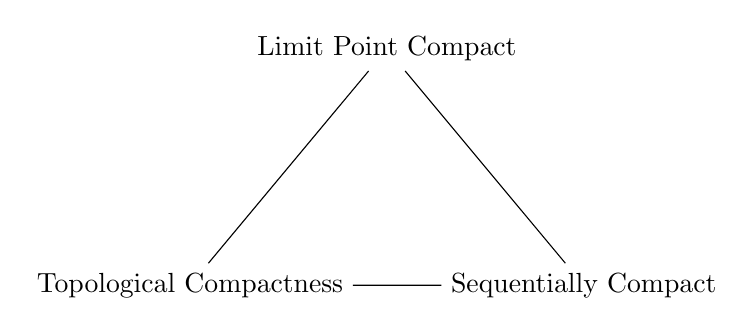
\begin{tikzpicture}
        % Define the nodes (vertices) with text
        \node (A) at (0,0) {Topological Compactness};
        \node (B) at (5,0) {Sequentially Compact};
        \node (C) at (2.5,3) {Limit Point Compact};

        % Draw the lines connecting the nodes to form a triangle
        \draw (A) -- (B) -- (C) -- cycle;
        \draw (A) -- (C);
    \end{tikzpicture}
\end{center}

\begin{enumerate}
    \item Topological Compactness: every open cover has a finite subcover.
    \item Sequentially Compact: every sequence has a convergent subsequence (think Bolzano-Weierstrass).
    \item Limit Point Compact: every infinite subset contains a limit point.
\end{enumerate}


\textcolor{Purple}{Theorem: Compact $\Longrightarrow$ Limit Point Compact}\\

\textbf{Proof:} Assume $K$ is compact and $E \subseteq K$ is infinite. For sake of contradiction, assume no point of $K$ is a limit point of $E$. Then, $\forall q \in K$, there exists a neighborhood $V_q$ of $q$ containing at most on point from $E$. Note that, if $q \in E$, this at most one point is $q$ itself. \\
Then $\{V_q\}_{q \in K}$ is an open cover of $K$. Since $K$ is compact, there exists a finite subcover $\{V_{q_i}\}_{i = 1}^n$. Then $E \subseteq K \subseteq \bigcup_{i=1}^nV_{q_i}$. But $E$ is infinite while $\bigcup_{i=1}^nV_{q_i}$ contains at most $n$ points from $E$. Then this is a contradiction, and thusly $q$ is a limit point of $E$.
$E$

\newpage

\subsection{Compactness in $\mathbb{R}^n$}

Note that the first two elements of the next theorem are known as the \textbf{\textcolor{ForestGreen}{Heine-Borel Theorem}}.

\textbf{Theorem:} If a set $E$ in $\mathbb{R}^n$ has one of the following three properties, then it has the other two:
\begin{enumerate}
    \item $E$ is closed and bounded.
    \item $E$ is compact.
    \item Every infinite subset of $E$ has a limit point in $E$.
\end{enumerate}

Note that this is just \textit{the Trinity} from the end of the previous section.\\

\textbf{Theorem: (Weierstrass)} Let $E \subseteq \mathbb{R}$ with $E$ bounded and infinite. Then $E$ has at least one limit point (this limit point is not necessarily contained in $E$).\\

\textbf{Proof:} First, since $E$ is bounded, $\exists M>0 \big| E \subseteq [-M,M]$. Note that at least one of the two sets $[-M,0]$ or $[0,M]$ contains infinitely many points of $E$. Then we will call this set containing these infinitely many points $[a,b]$. Similarly, at least one of $\biggl[a_1, \dfrac{a_1+b_1}{2} \biggr]$ or $\biggl[ \dfrac{a_1+b_1}{2}, b_1 \biggr]$ contains infinitely many points of $E$. Then we will call this set containing these infinitely many points $[a_2,b_2]$. Then we continue bisecting to obtain a sequence of nested intervals $[a_n,b_n]$. \\

Cantor's Intersection Theorem says that $x = \sup{\{a_n \big| n \in \mathbb{N}\}} \in \bigcap_{n \in \mathbb{N}} [a_n,b_n]$.\\

Now, we claim that this $x$ is a limit point of $E$. To show this, let $B_r(x)$ be a neighborhood of $x$. Now $b_n-a_n = \dfrac{M}{2^{n+1}} \longrightarrow 0$ as $n \longrightarrow \infty$. So $\exists N \in \mathbb{N} \big| b_N-a_N<r$. Then $[a_N,b_N] \subseteq B_r(x)$. Note that $[a_N,b_N]$ contains infinitely many points of $E$. Then we must have that $x \in E'$. $\square$\\

Note that it is left up to the reader to generalize this to $\mathbb{R}^n$. Rudin does this on page $40$ in his proof of \textbf{Theorem 2.42}. \\

\textbf{Corollary:} If $E \subseteq \mathbb{R}^n$ is closed, bounded, and infinite, then $E$ \textit{contains} at least one limit point.\\

\textbf{Corollary:} If $E \subseteq \mathbb{R}^n$ is closed and counded, then $E$ is limit point compact.\\

Note that the next theorem is not discussed in Rudin, but this method will very likely be useful during the comprehensive exam.\\

\textbf{Theorem: Lindel\"off Covering Theorem}\\
Let $E \subseteq \mathbb{R}^n$. Then every open cover of $E$ has a countable subcover.\\

\textbf{Proof:} Let $\Phi$ be an open cover of $E$, and let $\Psi=\{B_r(x) \big| r \in \mathbb{Q}, x \in \mathbb{Q}^n\} \cong \mathbb{Q}^{n+1}$. Note that $\Psi$ is countable, so we write
\begin{center}
    $\Psi = \{A_1, A_2, A_3, \dots\}$ with each $A_i$ an open ball. 
\end{center}
Now, let $x \in E$. Then there exists some open set $S \in \Phi$ such that $x \in S$. To get to the next step, first, we muct complete a mini proof inside the proof. We claim that there exists some $A_k \in \Psi$ such that $x \in A_k \subseteq S$. \\

Since $S$ is open and $x \in S$, we know there exists some open ball $B_r(x) \subseteq S$. Then, by the density of $\mathbb{Q}$ in $\mathbb{R}$, we choose $y \in \mathbb{Q}^n$ such that $y \in B_{\sfrac{r}{4}}(x)$ and $q \in \mathbb{Q}$ such that $\sfrac{r}{4} < q < \sfrac{r}{2}$. Further, note that $x \in B_q(y)$ and let $z \in B_q(y)$. Then $d(x,z) \leq d(y,z)+d(x,y)<q+\sfrac{r}{4}<\sfrac{r}{2}+\sfrac{r}{4}<r$. Thusly, $B_q(y) \subseteq B_r(x)$. But $B_q(y) \in \Psi$, so we must have that $B_q(y)=A_K$ for some $K \in \mathbb{N}$. \\

Now, if we let $x$ vary over $E$ we obtain a countable subcollection $\{A_{K_i}\}_{i \in \mathbb{N}}$ from $\Psi$ which covers $E$. Since each $A_{K_i}$ is contained in some $S_i \in \Phi$ (shown by the mini proof above), we must have that $\{S_i\}_{i \in \mathbb{N}}$ is a countable subcover of $\Phi$. $\square$\\

\textbf{Theorem: Heini-Borel}\\
A set in $\mathbb{R}^n$ is compact if and only if it is closed and bounded in $\mathbb{R}^n$.\\

\textbf{Proof:} The forward part of this proof is part of the homework. We will prove that compact implies closed and compact implies bounded.\\

For the other direction, assume $E \in \mathbb{R}^n$ is closed and bounded. Now, let $\Phi$ be an open cover of $E$. By Lindel\"off, there exist countable subcovers $A_1, A_2, A_3, \dots$. Let $S_m = \bigcup_{i=1}^m A_i$. Each $S_m$ is open and $E \subseteq \bigcup_{m \in \mathbb{N}}S_m = \bigcup_{i \in \mathbb{N}}A_i$. Let $Q_m = S_m^c \cap E$. Now, each $Q_m$ is closed and contained in $E$, so each $Q_m$ is also bounded. Further, $Q_{m+1} \subseteq Q_m$.\\

For sake of contradiction, assume $Q_m \neq \emptyset \ \forall m \in \mathbb{N}$. Let $x_m \in Q_m-Q_{m+1}$. Then $\{x_m\}_{m \in \mathbb{N}}$ is bounded and infinite, so $\{x_m\}_{m \in \mathbb{N}}$ has a limit point, say $x$, by Weierstrass. So every neighborhood of $x$ contains infinitely many points $x_m$, say all $m \geq N$ for some $N \in \mathbb{N}$. But $Q_N \subseteq Q_{N-1} \subseteq \cdots \subseteq Q_1$, so every neighborhood of $x$ meets $Q_m \ \forall m \in \mathbb{N}$. That is, the intersection of each $Q_m$  contains some point other than $x$. Then $x$ is a limit point of each $Q_m$. That is, $x \in Q_m' \ \forall m \in \mathbb{N}$. But each $Q_m$ is closed, so $x \in Q_m \ \forall m \in \mathbb{N}$. So

\begin{align*}
    x \in \bigcap_{m \in \mathbb{N}}Q_m &= \bigcap_{m \in \mathbb{N}} \bigl(S_m^c \cap E \bigr)\\
    &= E \cap \biggl( \bigcup_{m \in \mathbb{N}} S_m\biggr)^c.
\end{align*}

But this should be empty since $E \subseteq \bigcup_{m \in \mathbb{N}} S_m$, so we have a contradiction. Thus there exists some $M \in \mathbb{N}$ such that $Q_M = \emptyset$. So $E \subseteq S_M = \bigcup_{i=1}^MA_i$. Thus, $\bigcup_{i=1}^MA_i$ is a finite subcover of $\Phi$. $\square$

Recall, a subset $E \subseteq X$ is called perfect if $E= E'$.\\

\textbf{Theorem:} If a subset of the Euclidean space $P \subseteq \mathbb{R}^k$ is perfect and nonempty, then $P$ is uncountable.\\

Note that this proof won't be found on any exams, but it is still good to know.\\

\textbf{Proof:} Note that $P$ is perfect \textit{and} nonempty, so we must have that $\exists x \in P'$. But since finite sets have no limit points, we must have that $P$ is infinite. For sake of contradiction, assume $P = \{x_1, x_2, x_3, \dots \}$. Choose any neighborhood $B_{r_1}(x_1)$. Since $x_1 \in P$ and $P$ is perfect, we must have that $x_1 \in P'$. Then there exists some $y \in P \cap B_{r_1}(x_1)$ such that $y \neq x_1$.\\

Now, let $r_2 = \dfrac{1}{2} \min{\{d(x_1,y), r_1-d(x_1,y)\}}$. Note that the $\dfrac{1}{2}$ ensures that $x_1 \notin C_{r_2}(y)$ and $C_{r_2}(y) \subseteq B_{r_1}(x_1)$, while the $\min{\{d(x_1,y), r_1-d(x_1,y)\}}$ ensures that $B_{r_2}(y) \subseteq B_{r_1}(x_1)$. Note that there exists an open ball $B_{r_2}(y)$ such that 
\begin{enumerate}
    \item $\overline{B_{r_2}(y)} \subseteq B_{r_1}(x_1)$
    \item $x_1 \notin \overline{B_{r_2}(y)}$
    \item $B_{r_2}(y) \cap P \neq \emptyset$ with $y \in B_{r_2}(y) \cap P$.
\end{enumerate}

We then repeat this process to construct open balls such that 

\begin{enumerate}
    \item $\overline{B_{r_{n+1}}(y_n)} \subseteq B_{r_n}(x_n)$
    \item $x_n \notin \overline{B_{r_{n+1}}(y_n)}$
    \item $B_{r_{n+1}}(y_n) \cap P \neq \emptyset$.
\end{enumerate}

Now, let $K_n = \overline{B_{r_n}(x_n)} \cap P$. In particular, note that $x_n \notin K_{n+1} \ \forall x_n \in P$. So no point of $P$ lies in $\bigcap_{n = 1}^{\infty}K_n$. But since $K_n \subseteq P \ \forall n \in \mathbb{N}$, this says that 
\begin{center}
    $P \cap \bigcap_{n=1}^{\infty}K_n = \emptyset = \bigcap_{n=1}^{\infty}K_n$
\end{center}

which is a contradiction. Then we must have that $P$ cannot be enumerated (that is, $P \neq \{x_1, x_2, x_3, \dots\}$. Thusly, $P$ is uncountable. $\square$\\

Note that, since each $K_n$ is nonempty and compact, and since $K_n$ is a closed subset of compact $\overline{B_{r_n}(x_n)}$ (by Heine-Borel, since we're in $\mathbb{R}^k$), and since $K_{n+1} \subseteq K_n$. So, finally, by Cantor's Intersection theorem, $\bigcap_{n=1}^{\infty}K_n = \emptyset$. But this is the contradiction, so thusly $P$ is uncountable.\\

\textbf{Corollary:} Every closed interval $[a,b] \in \mathbb{R}$ is uncountable.\\

\textbf{Corollary:} $\mathbb{R}$ is uncountable.\\

\textcolor{NavyBlue}{Example:} Consider the Cantor (ternary) set. The idea is to iteratively delete the open middle third from a collection of intervals, starting with the interval $E_0=[0,1]$. Then we have
\begin{align*}
    E_0&=[0,1]\\
    E_1 &= \biggl[0, \dfrac{1}{3}\biggr] \cup \biggl[\dfrac{2}{3},1\biggr]\\
    E_2 &= \biggl[0, \dfrac{1}{9} \biggr] \cup \biggl[\dfrac{2}{9}, \dfrac{1}{3} \biggr] \cup \biggl[\dfrac{2}{3}, \dfrac{7}{9} \biggr] \cup \biggl[\dfrac{8}{9}, 1 \biggr] \\
    &\vdots \\
    E_n &= \dfrac{E_{n-1}}{3} \cup \biggl( \dfrac{2}{3}+\dfrac{E_{n-1}}{3} \biggr)
\end{align*}

Note that, when we say that we are dividing a set $E_i$ by some number, say $3$, we are really saying
\begin{center}
    $\dfrac{E_{n-1}}{3} = \biggl\{ \dfrac{e}{3} \bigg| e \in E_{n-1} \biggr\}$.
\end{center}

Then $E_n$ is the union of $2^n$ closed intervals with each interval having length $\biggl( \dfrac{1}{3} \biggr)^n$. Now, let $P = \bigcap_{n=1}^{\infty} E_n$. Then $P$ is the Cantor set. So we have

\begin{align*}
    P &= [0,1]- \bigcup_{n = 0}^{\infty} \bigcup_{k=1}^{3^n-1} \biggl( \dfrac{3k+1}{3^{n+1}}, \dfrac{3k+2}{3^{n+1}} \biggr) \\
    &= \bigcap_{n=1}^{\infty} \bigcup_{k=0}^{3^{n-1}-1} \biggl(\biggl[ \dfrac{3k}{3^n}, \dfrac{3k+1}{3^n} \biggr] \bigcup \biggl[ \dfrac{3k+2}{3^n}, \dfrac{3k+3}{3^n} \biggr]  \biggr)
\end{align*}

Note that, in the first equality for $P$ above, the first union represents the row (that is, the $n$ that is the subscript of $E$), while the second union represents the column (that is, the second union is the piece from each row that is removed). \\

Note that endpoints are never removed from the Cantor set (since we are removing \textit{open} middle thirds). Then we must have that $0, \dfrac{1}{3}, \dfrac{7}{9}$, etc. are always in $P$. But also, we have $\dfrac{1}{4} \in P$. Most points in $P$ are irrational, as $P$ is uncountable.\\

Another way that we describe $P$ is to say

\begin{center}
    $P = \{x \in [0,1] \big| \text{base }5 \text{ expansion of }x \text{ only contains the digits }0 \text{ and } 2\}$.
\end{center}

Consider the following about the Cantor set:

\begin{enumerate}
    \item Perfect (\textit{this has been a comp question in the past})
    \item Uncountable
    \item Measure zero (\textit{that is, it has zero length}). Note that we deleted $\sum_{n = 0}^{\infty}\dfrac{2^n}{3^{n+1}}$, where the numerator is the number of intervals and the denominator is the length of each interval. Notice that this is a convergent geometric series that converges to 1.
    \item Compact (by Heine-Borel)
    \item A fractal
    \item Totally disconnected (contains no intervals and has no nontrivial connected subsets)
    \item Nowhere dense (the interior of it's closure is empty, i.e. $(\overline{P})^{\circ} = \emptyset \Longrightarrow  ((\overline{P})^{\circ})^c$ is dense)
    \item The only totally disconnected perfect compact metric space
    \item $P+P = [0,2]$. This is useless, but surprising.
\end{enumerate}


\textbf{Theorem:} The Cantor set, $P$, is perfect.\\

\textbf{Proof:} $P$ is closed \textit{(show this)}, so we have that $P' \subseteq P$. Then we need only show that $P \subseteq P'$. Let $x \in P$ and let $S$ be some open neighborhood of $x$. Let $E_n$ be a collection of $2^n$ closed intervals such that $P = \bigcap_{n \in \mathbb{N}} E_n$ with each closed interval in $E_n$ denoted $I_n$ for some $n \in \mathbb{N}$. \\

Now, choose $n$ large enough such that $I_n \subseteq S$. Note that $I_n$ has length $\dfrac{1}{3^n}$, so the larger our $n$, the smaller our interval. Let $y$ be an endpoint of $I_n$ with $y \neq x$. Then $x \in P'$ and thusly, $P \subseteq P'$, so $P = P'$ and $P$ is perfect. $\square$\\

\newpage

\subsection{Connected Sets}

\textbf{Definition:} Let $A, B \subseteq X$ with $X$ a metric space.
\begin{enumerate}
    \item Then $A$ and $B$ are \textcolor{ForestGreen}{separated} if $A \cap \overline{B} = \overline{A} \cap B = \emptyset$. \textit{Note that this is stronger than disjoint, which says only that $A \cap B = \emptyset$.}
    \item A set $E \subseteq X$ is \textcolor{ForestGreen}{connected} if $E$ is not a union of two nonempty separated sets.
\end{enumerate}

\textcolor{NavyBlue}{Examples:}
\begin{enumerate}
    \item $A=(0,1)$ and $B=[1,2]$ are \textit{not} separated. Note that 
    \begin{align*}
        \overline{B} = B &\Longrightarrow A \cap B = A \cap \overline{B} = \emptyset \\
        \overline{A} = [0,1] &\Longrightarrow \overline{A} \cap B = \{1\} \neq \emptyset.
    \end{align*}
    \item Let $A = [0,1]$ and $B = [2,3]$. Then $E = A \cup B$ is \textit{not} connected, since $E$ \textit{is} a union of two nonempty separated sets. $A$ and $B$ are separated since $A \cap \overline{B} = \emptyset = \overline{A} \cap B$.
    \item Let $A = (0,1)$ and $B = (1,2)$. Then $E = A \cup B$ is \textit{not} connected. Note that $\overline{A} = [0,1]$ and $\overline{B} = [1,2]$, so $\overline{A} \cap B = \emptyset = A \cap \overline{B}$.
    \item $\mathbb{Q}$ is \textit{not} connected. Consider $A = (-\infty, \sqrt{2}) \cap \mathbb{Q}$ and $B = (\sqrt{2}, \infty) \cap \mathbb{Q}$. Then $A$ and $B$ form a separation of $\mathbb{Q}$. First, note that $\overline{A} = (-\infty,\sqrt{2}] \cap \mathbb{Q}$ and $\overline{B} = [\sqrt{2}, \infty) \cap \mathbb{Q}$. Then we have
    \begin{align*}
        \overline{A} \cap B &= (-\infty, \sqrt{2}] \cap \mathbb{Q} \cap (\sqrt{2}, \infty) \\
        A \cap \overline{B} &= (-\infty, \sqrt{2}) \cap \mathbb{Q} \cap [\sqrt{2}, \infty).
    \end{align*}
\end{enumerate}

\textbf{Theorem:} A set $E \subseteq \mathbb{R}$ is connected if and only if $x,y \in E$ and $x < z < y \Longrightarrow z \in E$. \textit{Note that this is a common comprehensive exam question.}\\

\textit{Proof:} We will prove by contrapositive. Then assume there exist some $x,y \in E$ with $x < z < y$ such that $z \notin E$. Let $A = E \cap (-\infty, z)$ and $B = E \cap (z, \infty)$. This forms a separation as $E = A \cup B$ and $A, B \neq \emptyset$ since $x \in A$ and $y \in B$. Specifically, note that 
\begin{align*}
    \overline{A} = E \cap (-\infty, z] &\Longrightarrow \overline{A} \cap B = (-\infty, z] \cap E \cap (z, \infty) \\
    \overline{B} = E \cap [z, \infty) &\Longrightarrow A \cap \overline{B} = (-\infty ,z) \cap E \cap [z, \infty). 
\end{align*}

Then it is clear that $E$ is the union of two nonempty separated sets and thus $E$ is \textit{not} connected. \\

For the other direction, assume $E$ is disconnected. Then we need to show there exists $x, y \in E$ and $z \in \mathbb{R}$ such that $x < z < y$ with $z \notin E$. Since $E$ is disconnected, there exists some separation $E = A \cup B$. Let $x,y \in E$ and, without loss of generality, $x < y$. Now, choose $x \in A$ and $y \in B$. Let $z = \sup{(A \cap [x,y])}$. Then $z \in \overline{A \cap [x,y]} \subseteq \overline{A} \cap [x,y]$. Then $z \in \overline{A}$, so we must have (by definition of separation) $z \notin B$. Then $z \neq y$. Also, $z \in [x,y]$, so we must have that $x \leq z < y$. Note that we still need to show that $z \neq x$. Then we consider two cases:
\begin{enumerate}
    \item If $z \notin A$, then $z \neq x$ since $x \in A$. Then $x < z < y$, so $z \notin A \cup B$ and we are done.
    \item If $z \in A$, then $z \notin \overline{B}$. In particular, $z \notin B'$. Then there exists some neighborhood of $z$ containing no points from $B$, say $(z-r,z+r)$. Let $z_1=z+\dfrac{r}{2}$. Then $z_1 \notin B$ and $z_1 < y$ (\textit{otherwise $y \in B \cap (z-r,z+r)$ which is not possible}). Then $x \leq z < z_1 < y \Longrightarrow x < z_1 < y$. \\
    Note that $z_1 \notin A$, or else $z_1 \in A \cap [x,y]$. But $z_1 > \sup{(A \cap [x,y])}$, which would be a contradiction. Whencely, $z_1 \notin A \cup B \Longrightarrow z_1 \notin E$. $\square$
\end{enumerate}

\textbf{Theorem:} $E$ is connected if and only if the only subsets of $E$ which are clopen are $E$ and $\emptyset$.

\textbf{Corollary:} $\mathbb{Q}$ is not connected $\Longrightarrow \exists \text{ nonempty } A \subsetneq \mathbb{Q}$ such that $A$ is clopen.

\end{document}
